\begin{frame}[label=appendix-recording-setup]{Appendix - Recording Simulation Setup}
\transfade[duration=0.25]
\vspace{-0.08cm}
\begin{outlinecard}[Simulation Environment]
  \begin{columns}[T,onlytextwidth]
    \begin{column}{0.5\textwidth}
      \centering
      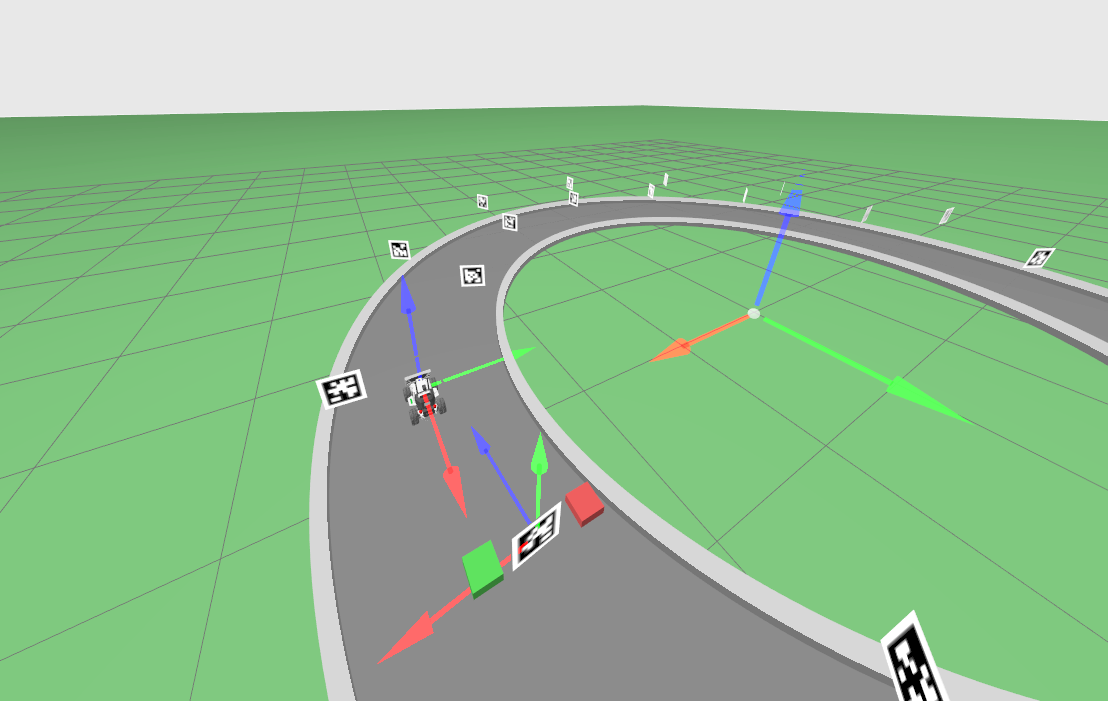
\includegraphics[width=0.96\linewidth,height=0.30\textheight,keepaspectratio]{../Report/Images/limo_simulation_environment.png}\\[-0.5mm]
      {\tiny Gazebo scenario with fixed AprilTags}
    \end{column}
    \begin{column}{0.5\textwidth}
      \centering
      \only<3->{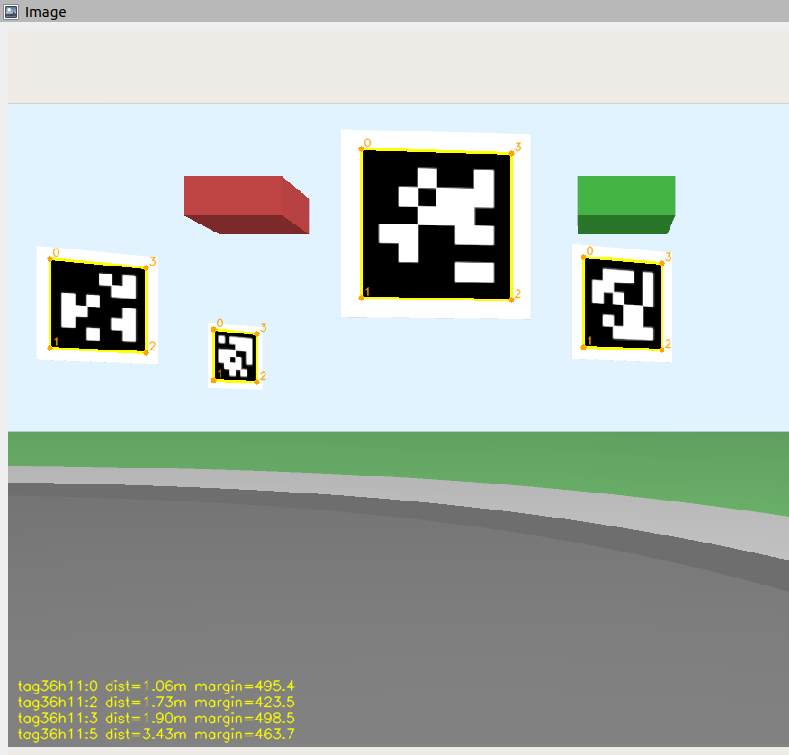
\includegraphics[width=0.96\linewidth,height=0.30\textheight,keepaspectratio]{../Report/Images/apriltag_detection_sim.png}\\[-0.5mm]}
      \only<3->{\tiny Simulated AprilTag detection input}
    \end{column}
  \end{columns}
\end{outlinecard}

\vspace{-0.05cm}
\begin{outlinecard}[Recording Inputs]
  \scriptsize
  \begin{itemize}
    \item<1-> Initial traversal logged into \texttt{rosbag2}.
    \item<2-> Camera intrinsics and AprilTag detections are stored frame-by-frame.
    \item<3-> This dataset feeds the offline map-and-trajectory reconstruction.
  \end{itemize}
\end{outlinecard}
\end{frame}

\edef\SimulationVideoFile{\detokenize{assets/simulation_validation.mp4}}
\edef\SimulationPosterFile{\detokenize{assets/simulation_validation_thumb.jpg}}
\edef\SimulationGraphPdfFile{\detokenize{../Report/svg-inkscape/sim_perception_gt_01_outputs_global_stride2__recording_trajectory_with_detected_and_groundtruth_tags_svg-raw.pdf}}
\colorlet{ValidationFrameColor}{NavyBlue}


\begin{frame}[label=appendix-synth-noisefree]{Optimized tag map and reconstructed camera trajectory in the noise-free scenario.}
\vspace{-0.08cm}
\centering
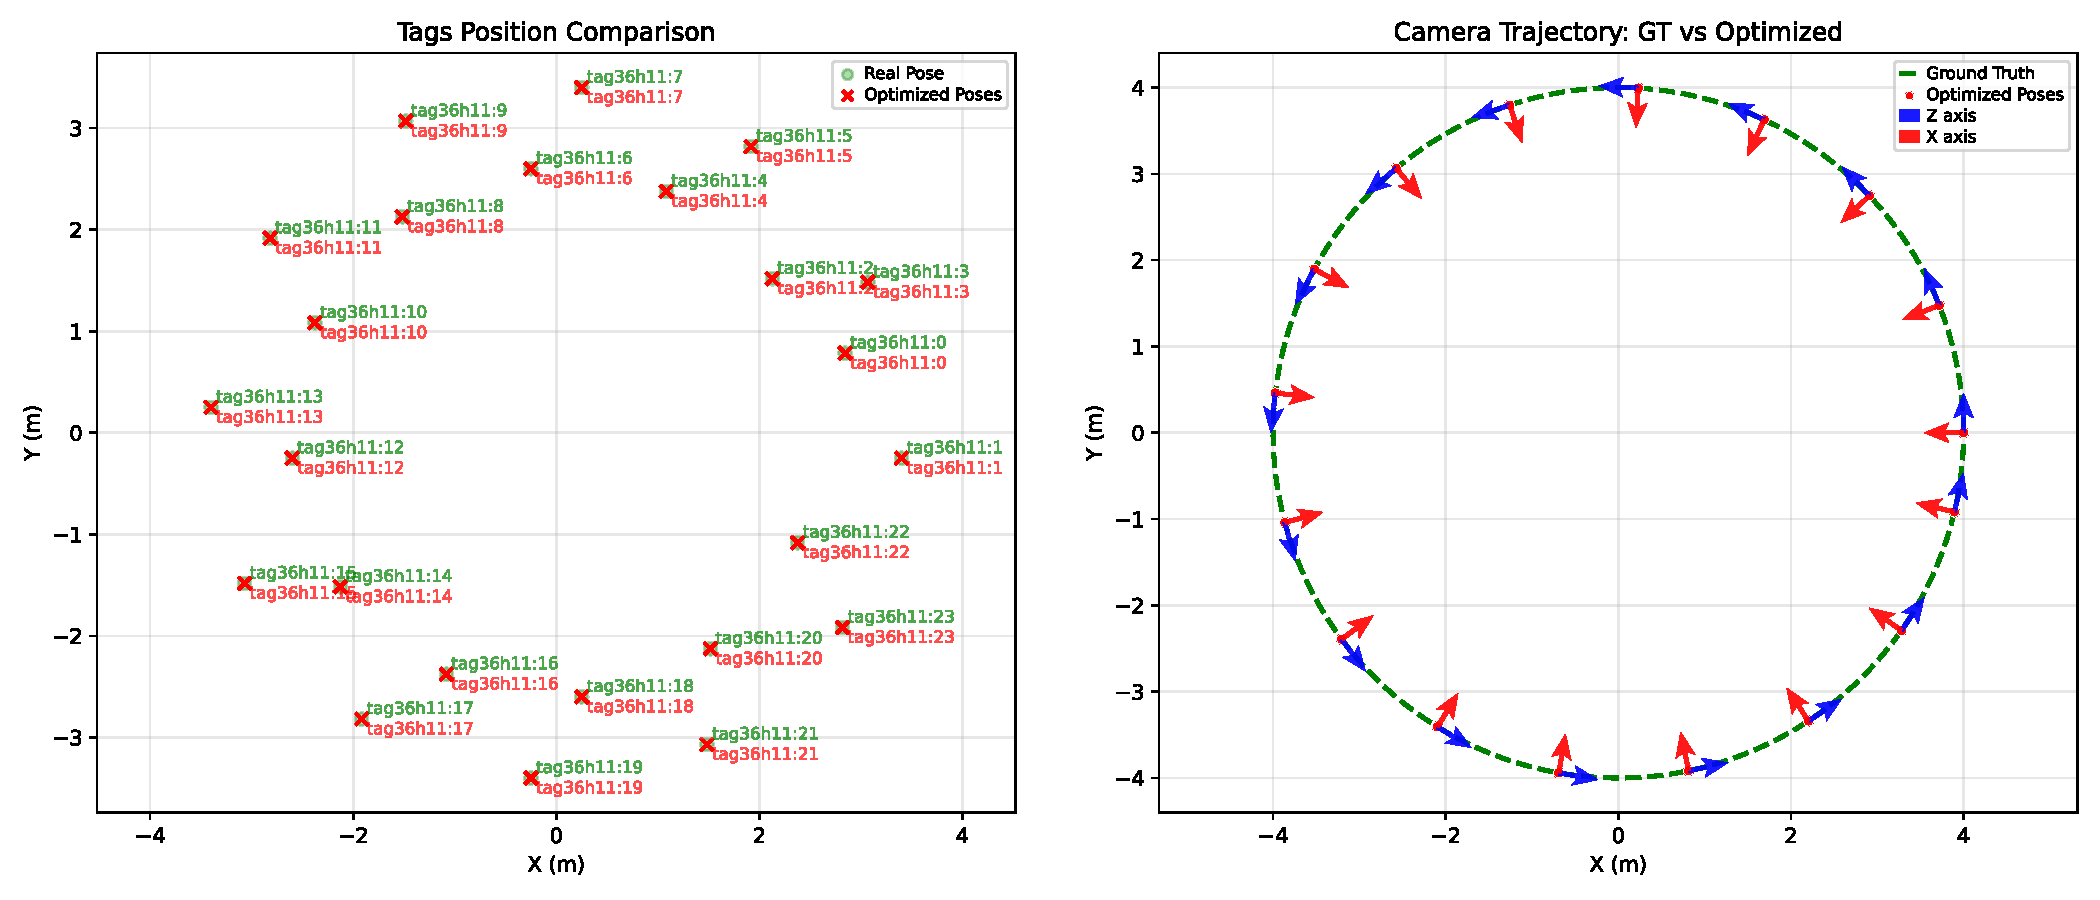
\includegraphics[width=0.92\linewidth,height=0.72\textheight,keepaspectratio]{../Report/svg-inkscape/comparison_optimized_lm_svg-raw.pdf}
\end{frame}

\begin{frame}[label=appendix-synth-noisy]{Optimized tag map and reconstructed trajectory under 10 cm Gaussian noise.}
\vspace{-0.08cm}
\centering
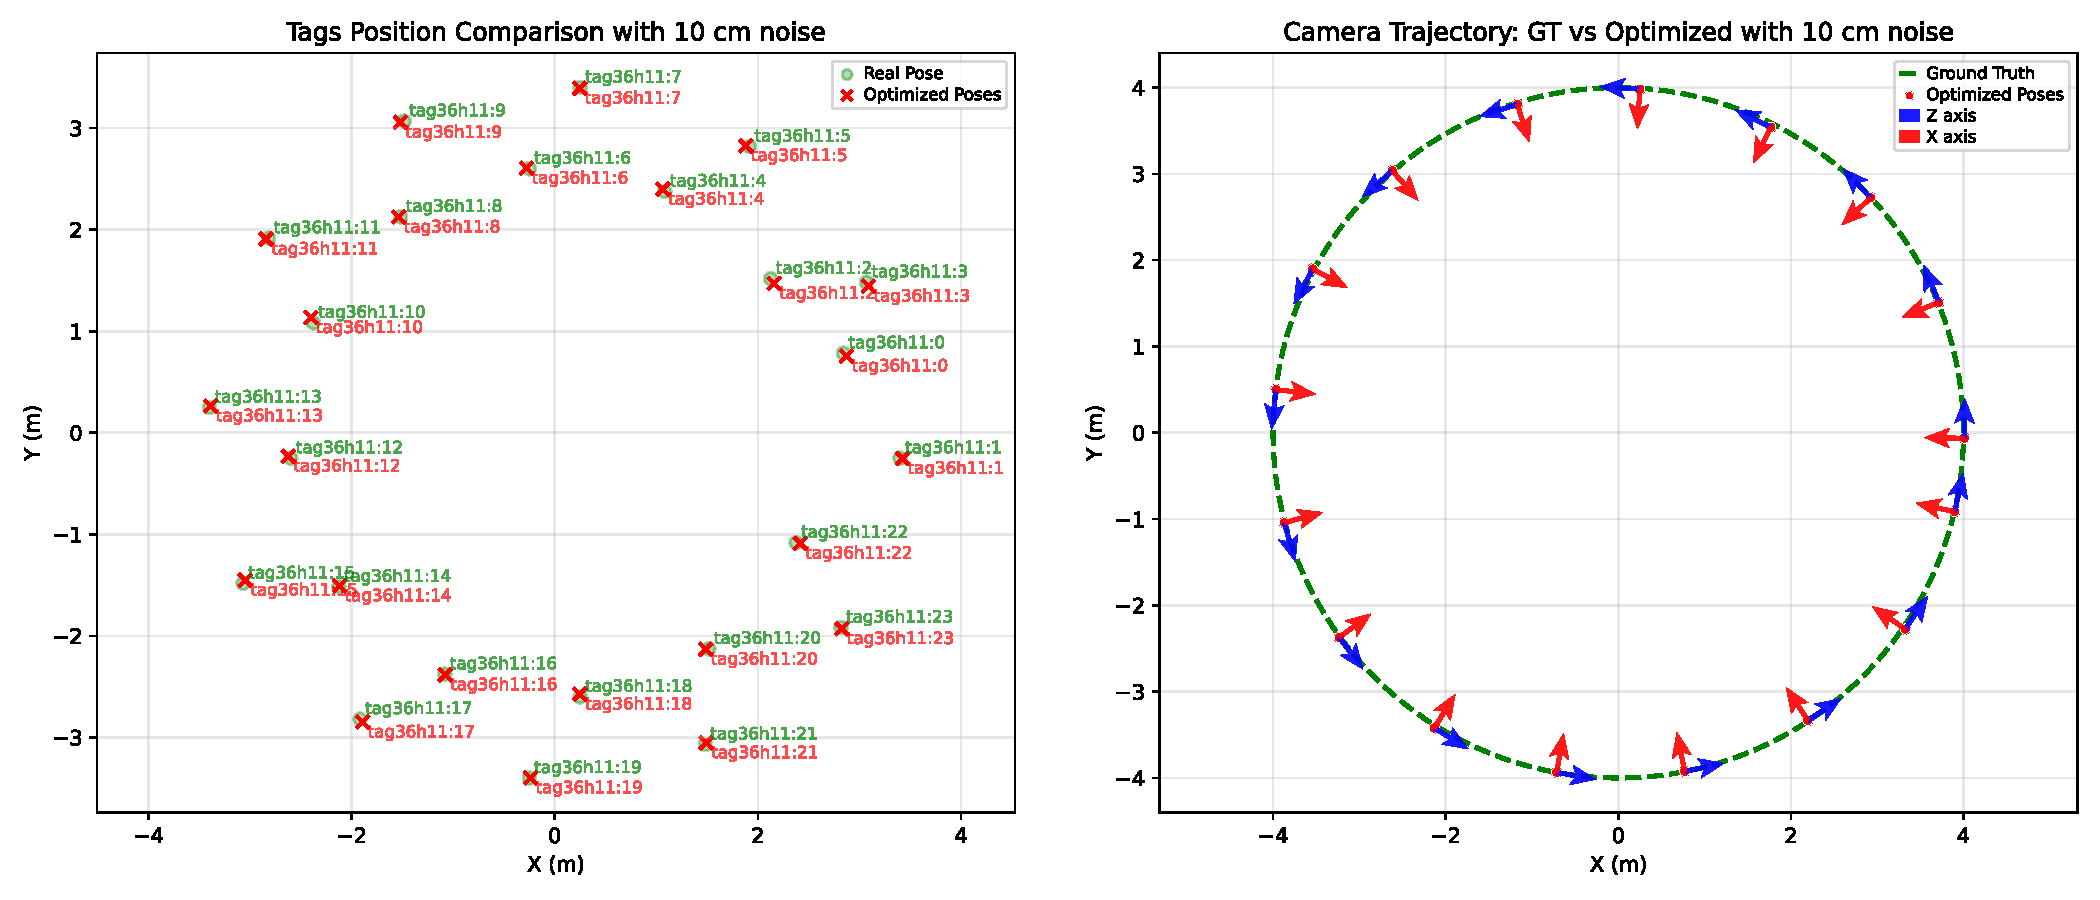
\includegraphics[width=0.92\linewidth,height=0.72\textheight,keepaspectratio]{../Report/svg-inkscape/comparison_optimized_lm_noise_10cm_svg-raw.pdf}
\end{frame}

\begin{frame}[label=appendix-mosaic-architecture]{Physical and simulated setups used to evaluate the proposed architecture.}
  \begin{columns}[c,onlytextwidth]
    \begin{column}{0.49\textwidth}
      \centering
      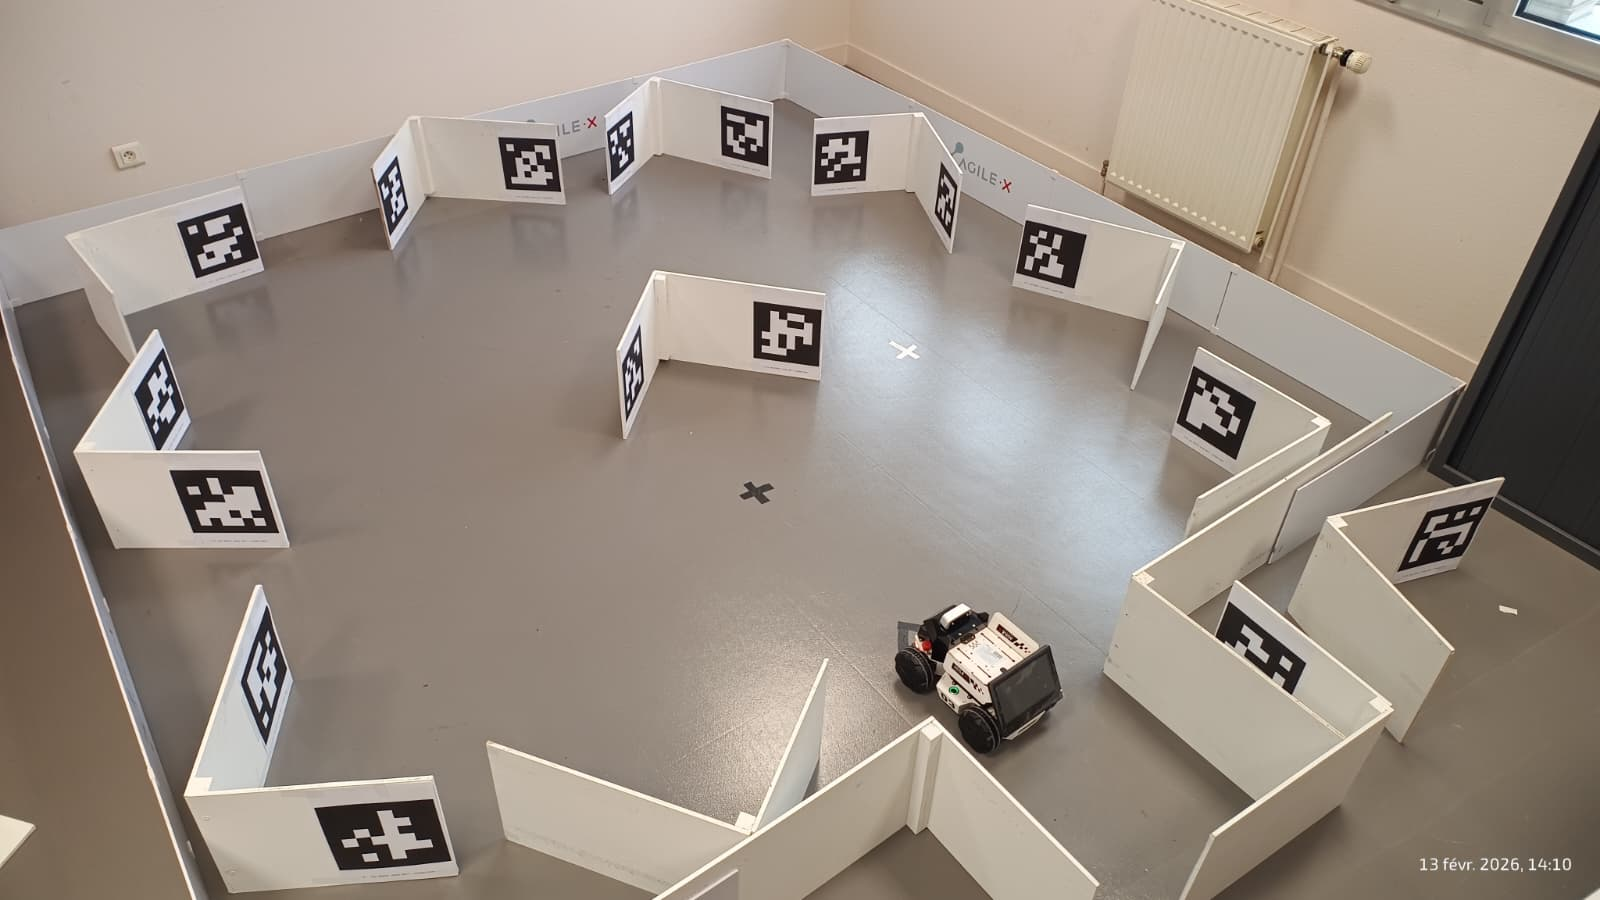
\includegraphics[width=\linewidth,height=0.65\textheight,keepaspectratio]{../Report/Images/limo_real_environment.png}
    \end{column}
    \begin{column}{0.49\textwidth}
      \centering
      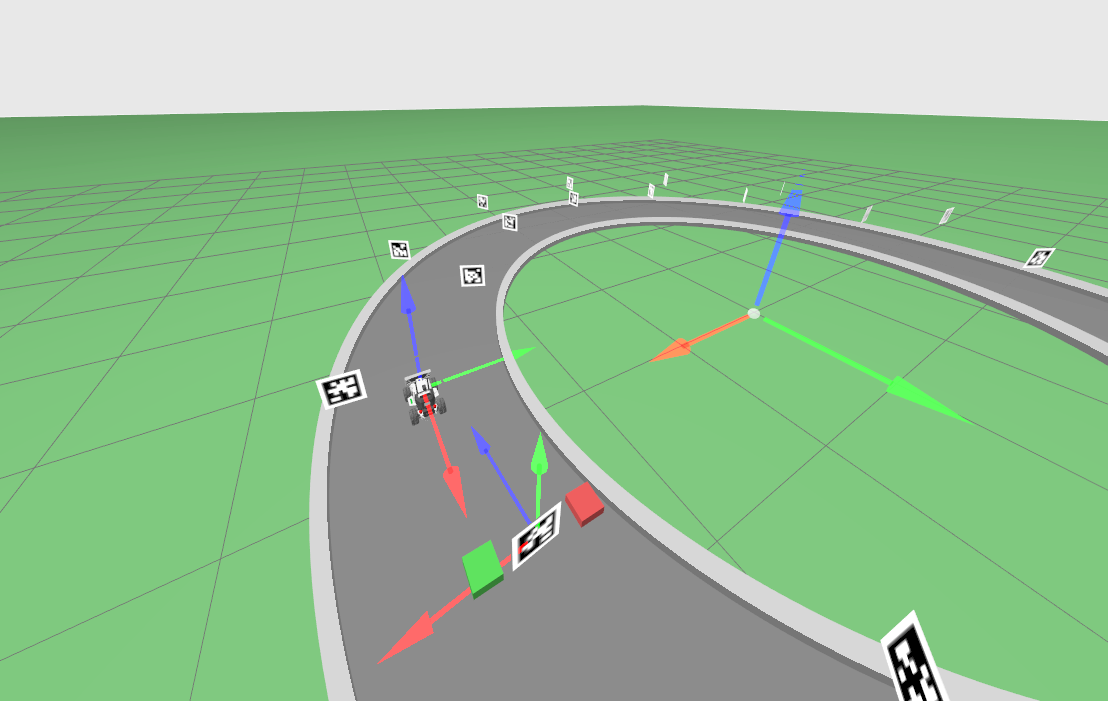
\includegraphics[width=\linewidth,height=0.65\textheight,keepaspectratio]{../Report/Images/limo_simulation_environment.png}
    \end{column}
  \end{columns}
\end{frame}

\begin{frame}[label=appendix-mosaic-detection]{Representative detection, each detected tag yields a camera-relative pose estimate obtained through a PnP formulation.}
  \begin{columns}[c,onlytextwidth]
    \begin{column}{0.49\textwidth}
      \centering
      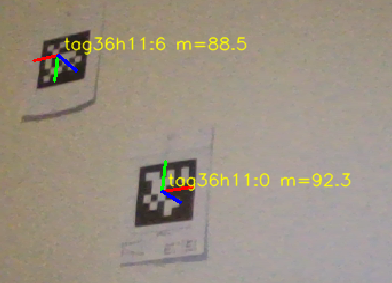
\includegraphics[width=0.96\linewidth,height=0.58\textheight,keepaspectratio]{../Report/Images/apriltag_detection_real.png}
    \end{column}
    \begin{column}{0.49\textwidth}
      \centering
      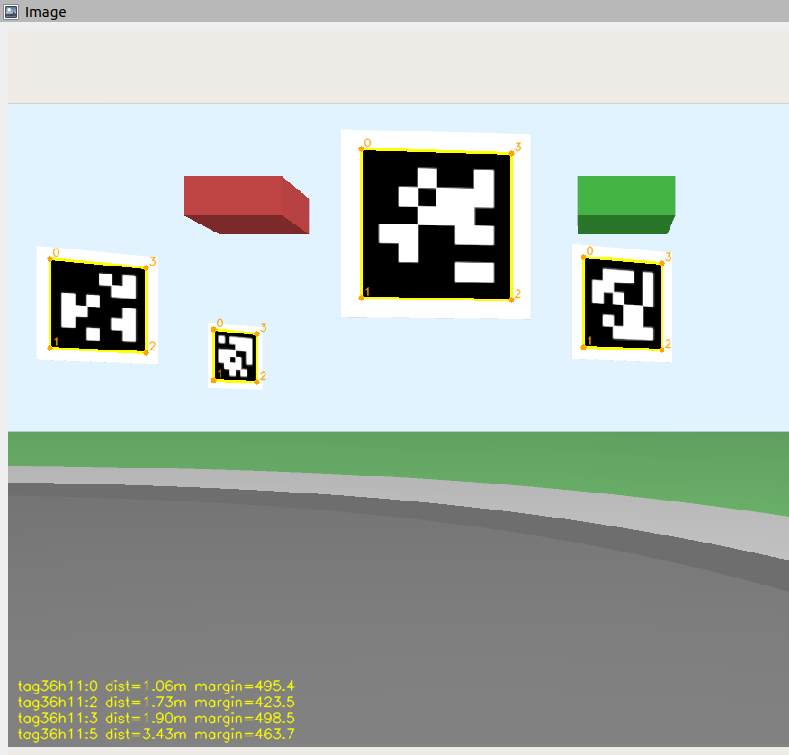
\includegraphics[width=0.96\linewidth,height=0.58\textheight,keepaspectratio]{../Report/Images/apriltag_detection_sim.png}
    \end{column}
  \end{columns}
\end{frame}

\begin{frame}[label=appendix-mosaic-rec-traj]{Reconstructed camera trajectory obtained after map optimization.}
  \begin{columns}[c,onlytextwidth]
    \begin{column}{0.49\textwidth}
      \centering
      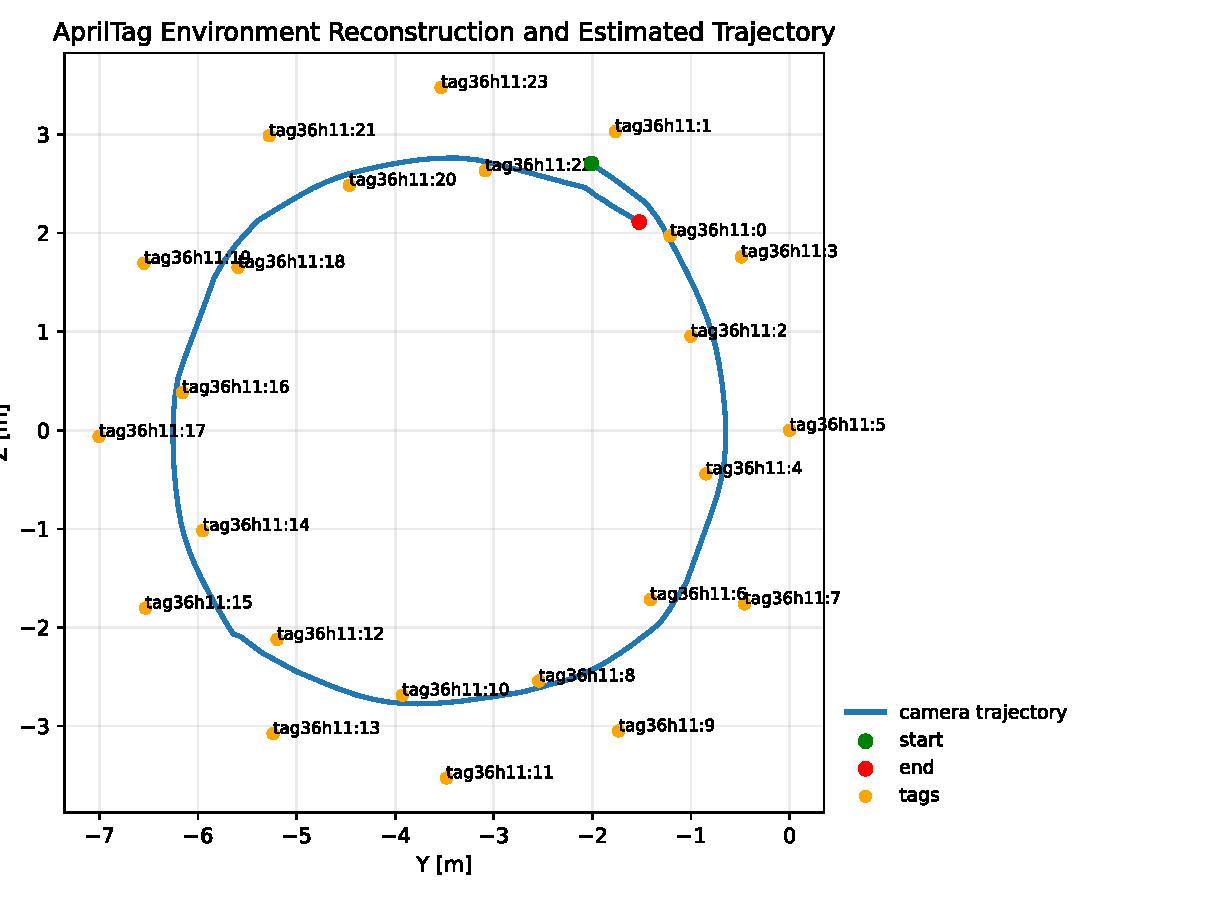
\includegraphics[width=\linewidth,height=0.65\textheight,keepaspectratio]{../Report/svg-inkscape/sim_perception_gt_01_outputs_global_stride2__recording_trajectory_basic_svg-raw.pdf}
    \end{column}
    \begin{column}{0.49\textwidth}
      \centering
      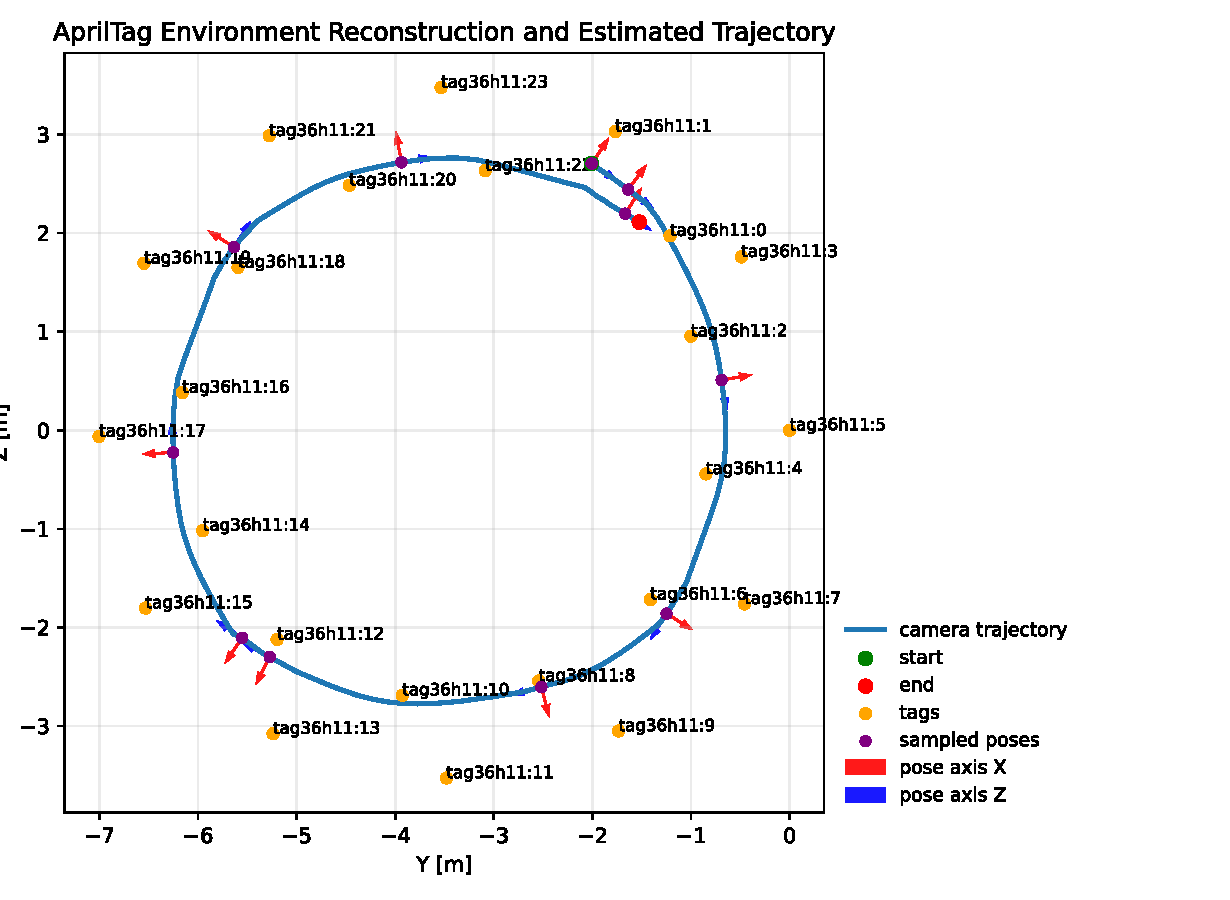
\includegraphics[width=\linewidth,height=0.65\textheight,keepaspectratio]{../Report/svg-inkscape/sim_perception_gt_01_outputs_global_stride2__recording_trajectory_with_axes_svg-raw.pdf}
    \end{column}
  \end{columns}
\end{frame}

\begin{frame}[label=appendix-mosaic-compare-gt]{Comparison between optimized reconstruction and ground-truth configuration.}
  \begin{columns}[c,onlytextwidth]
    \begin{column}{0.49\textwidth}
      \centering
      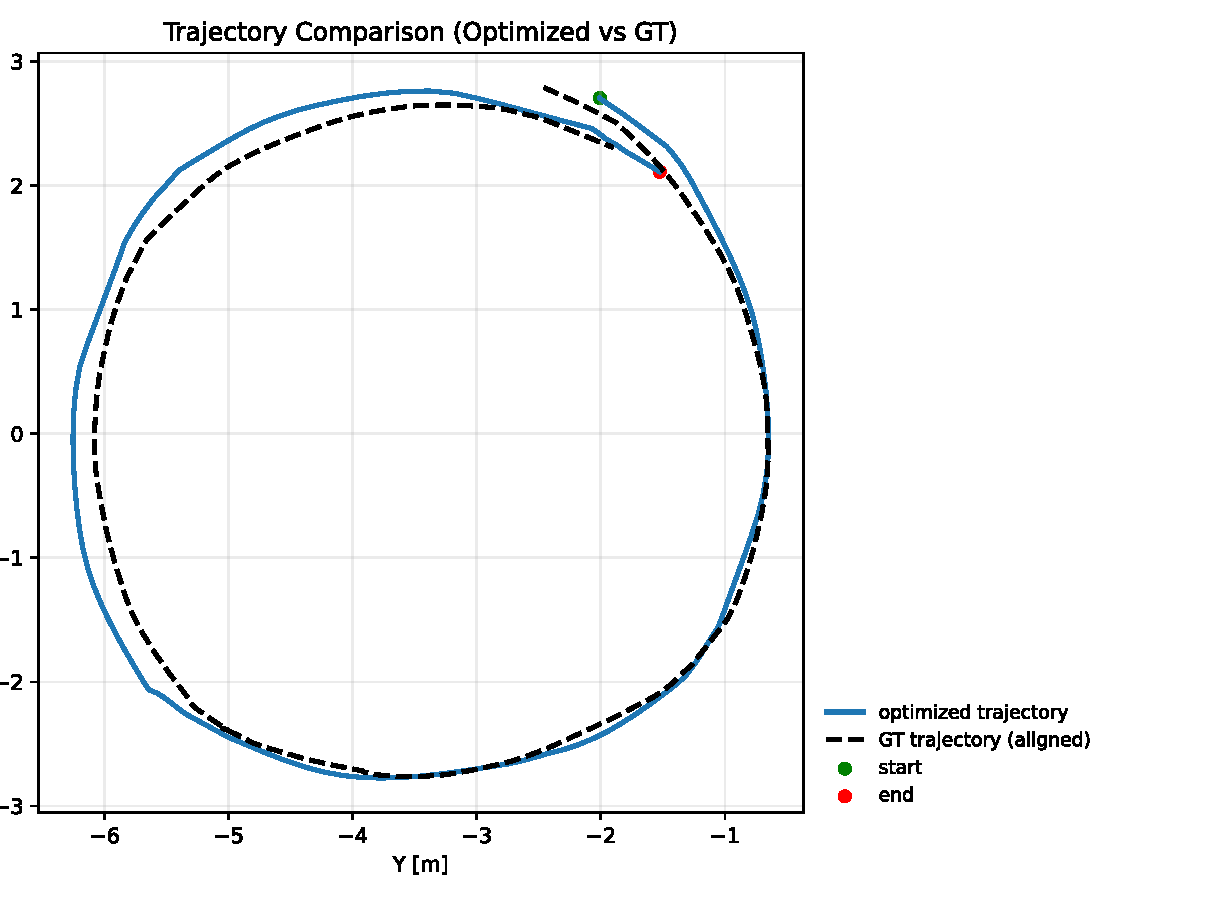
\includegraphics[width=\linewidth,height=0.65\textheight,keepaspectratio]{../Report/svg-inkscape/sim_perception_gt_01_outputs_global_stride2__recording_trajectory_comparison_optimized_vs_gt_svg-raw.pdf}
    \end{column}
    \begin{column}{0.49\textwidth}
      \centering
      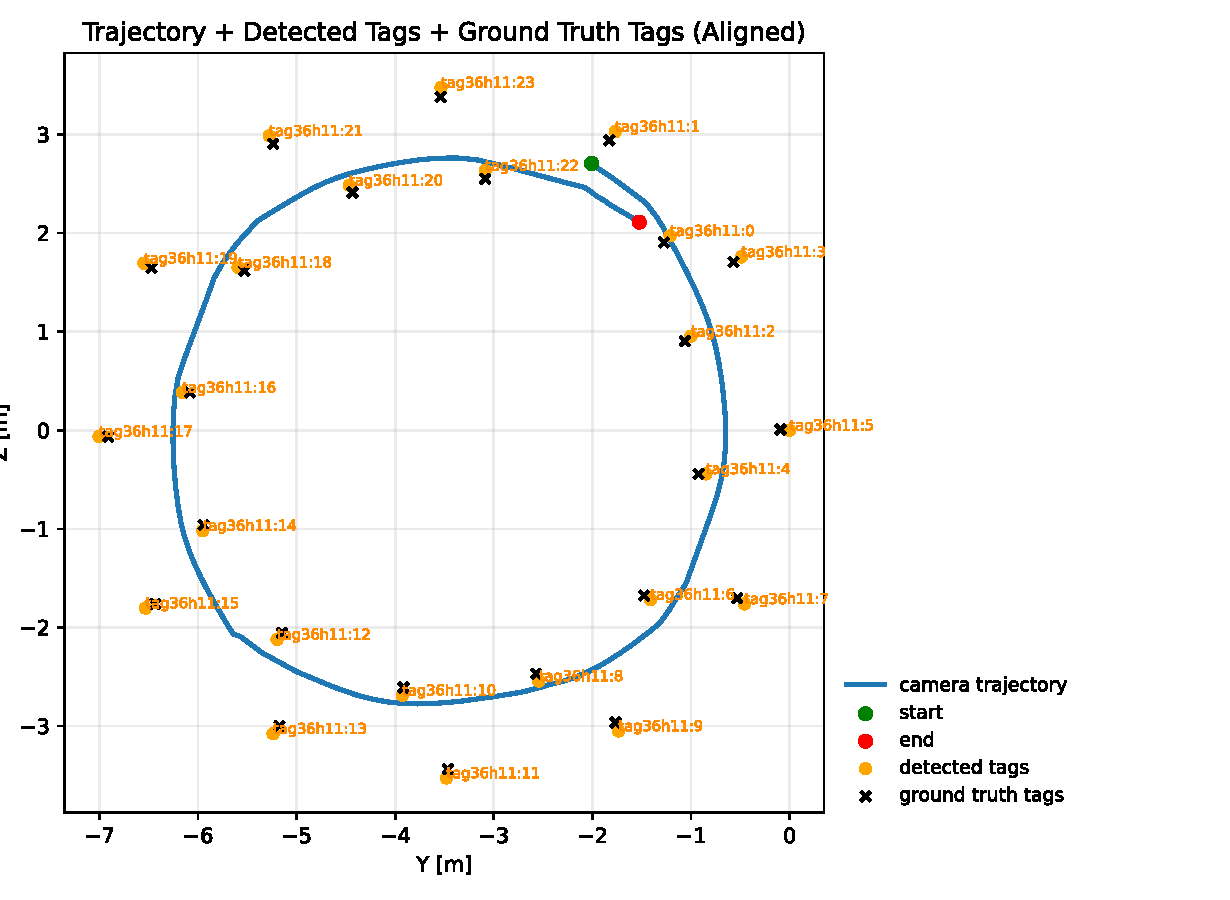
\includegraphics[width=\linewidth,height=0.65\textheight,keepaspectratio]{../Report/svg-inkscape/sim_perception_gt_01_outputs_global_stride2__recording_trajectory_with_detected_and_groundtruth_tags_svg-raw.pdf}
    \end{column}
  \end{columns}
\end{frame}

\begin{frame}[label=appendix-mosaic-synth-points]{Representative synthetic points used to validate the computation of $D$ in the YZ plane.}
  \begin{columns}[c,onlytextwidth]
    \begin{column}{0.49\textwidth}
      \centering
      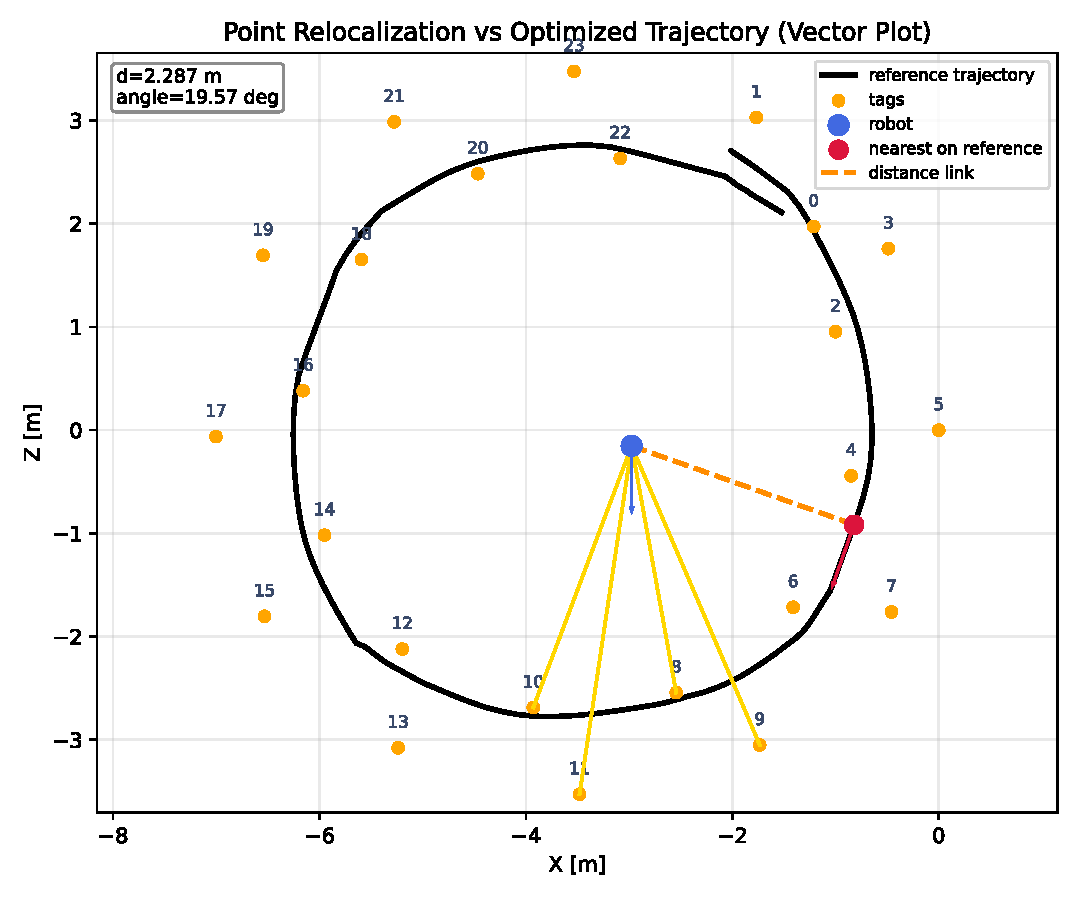
\includegraphics[width=\linewidth,height=0.65\textheight,keepaspectratio]{../Report/svg-inkscape/output_sim_between_tags_yz_01__relocalization_point_didactic_svg-raw.pdf}
    \end{column}
    \begin{column}{0.49\textwidth}
      \centering
      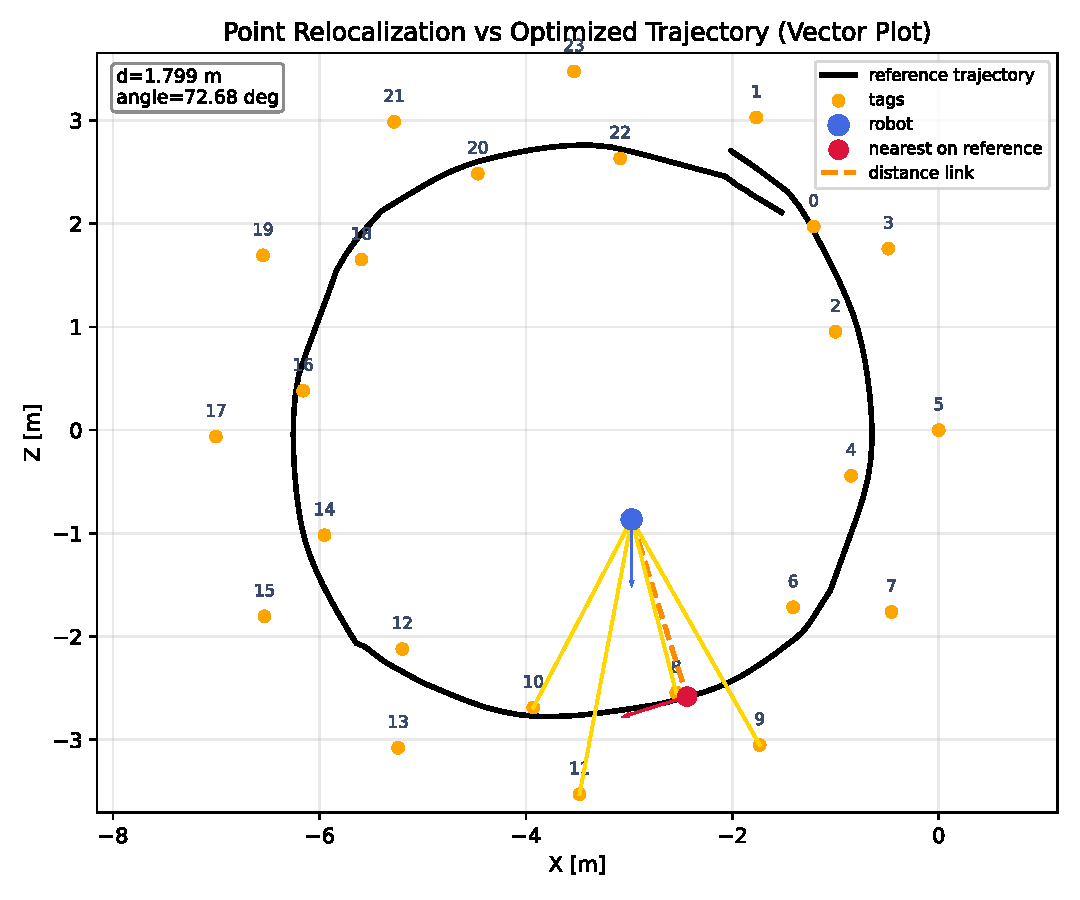
\includegraphics[width=\linewidth,height=0.65\textheight,keepaspectratio]{../Report/svg-inkscape/output_sim_between_tags_yz_08__relocalization_point_didactic_svg-raw.pdf}
    \end{column}
  \end{columns}
\end{frame}

\begin{frame}[label=appendix-mosaic-real-recording]{Real recording setup and corresponding reconstructed trajectory result.}
  \begin{columns}[c,onlytextwidth]
    \begin{column}{0.49\textwidth}
      \centering
      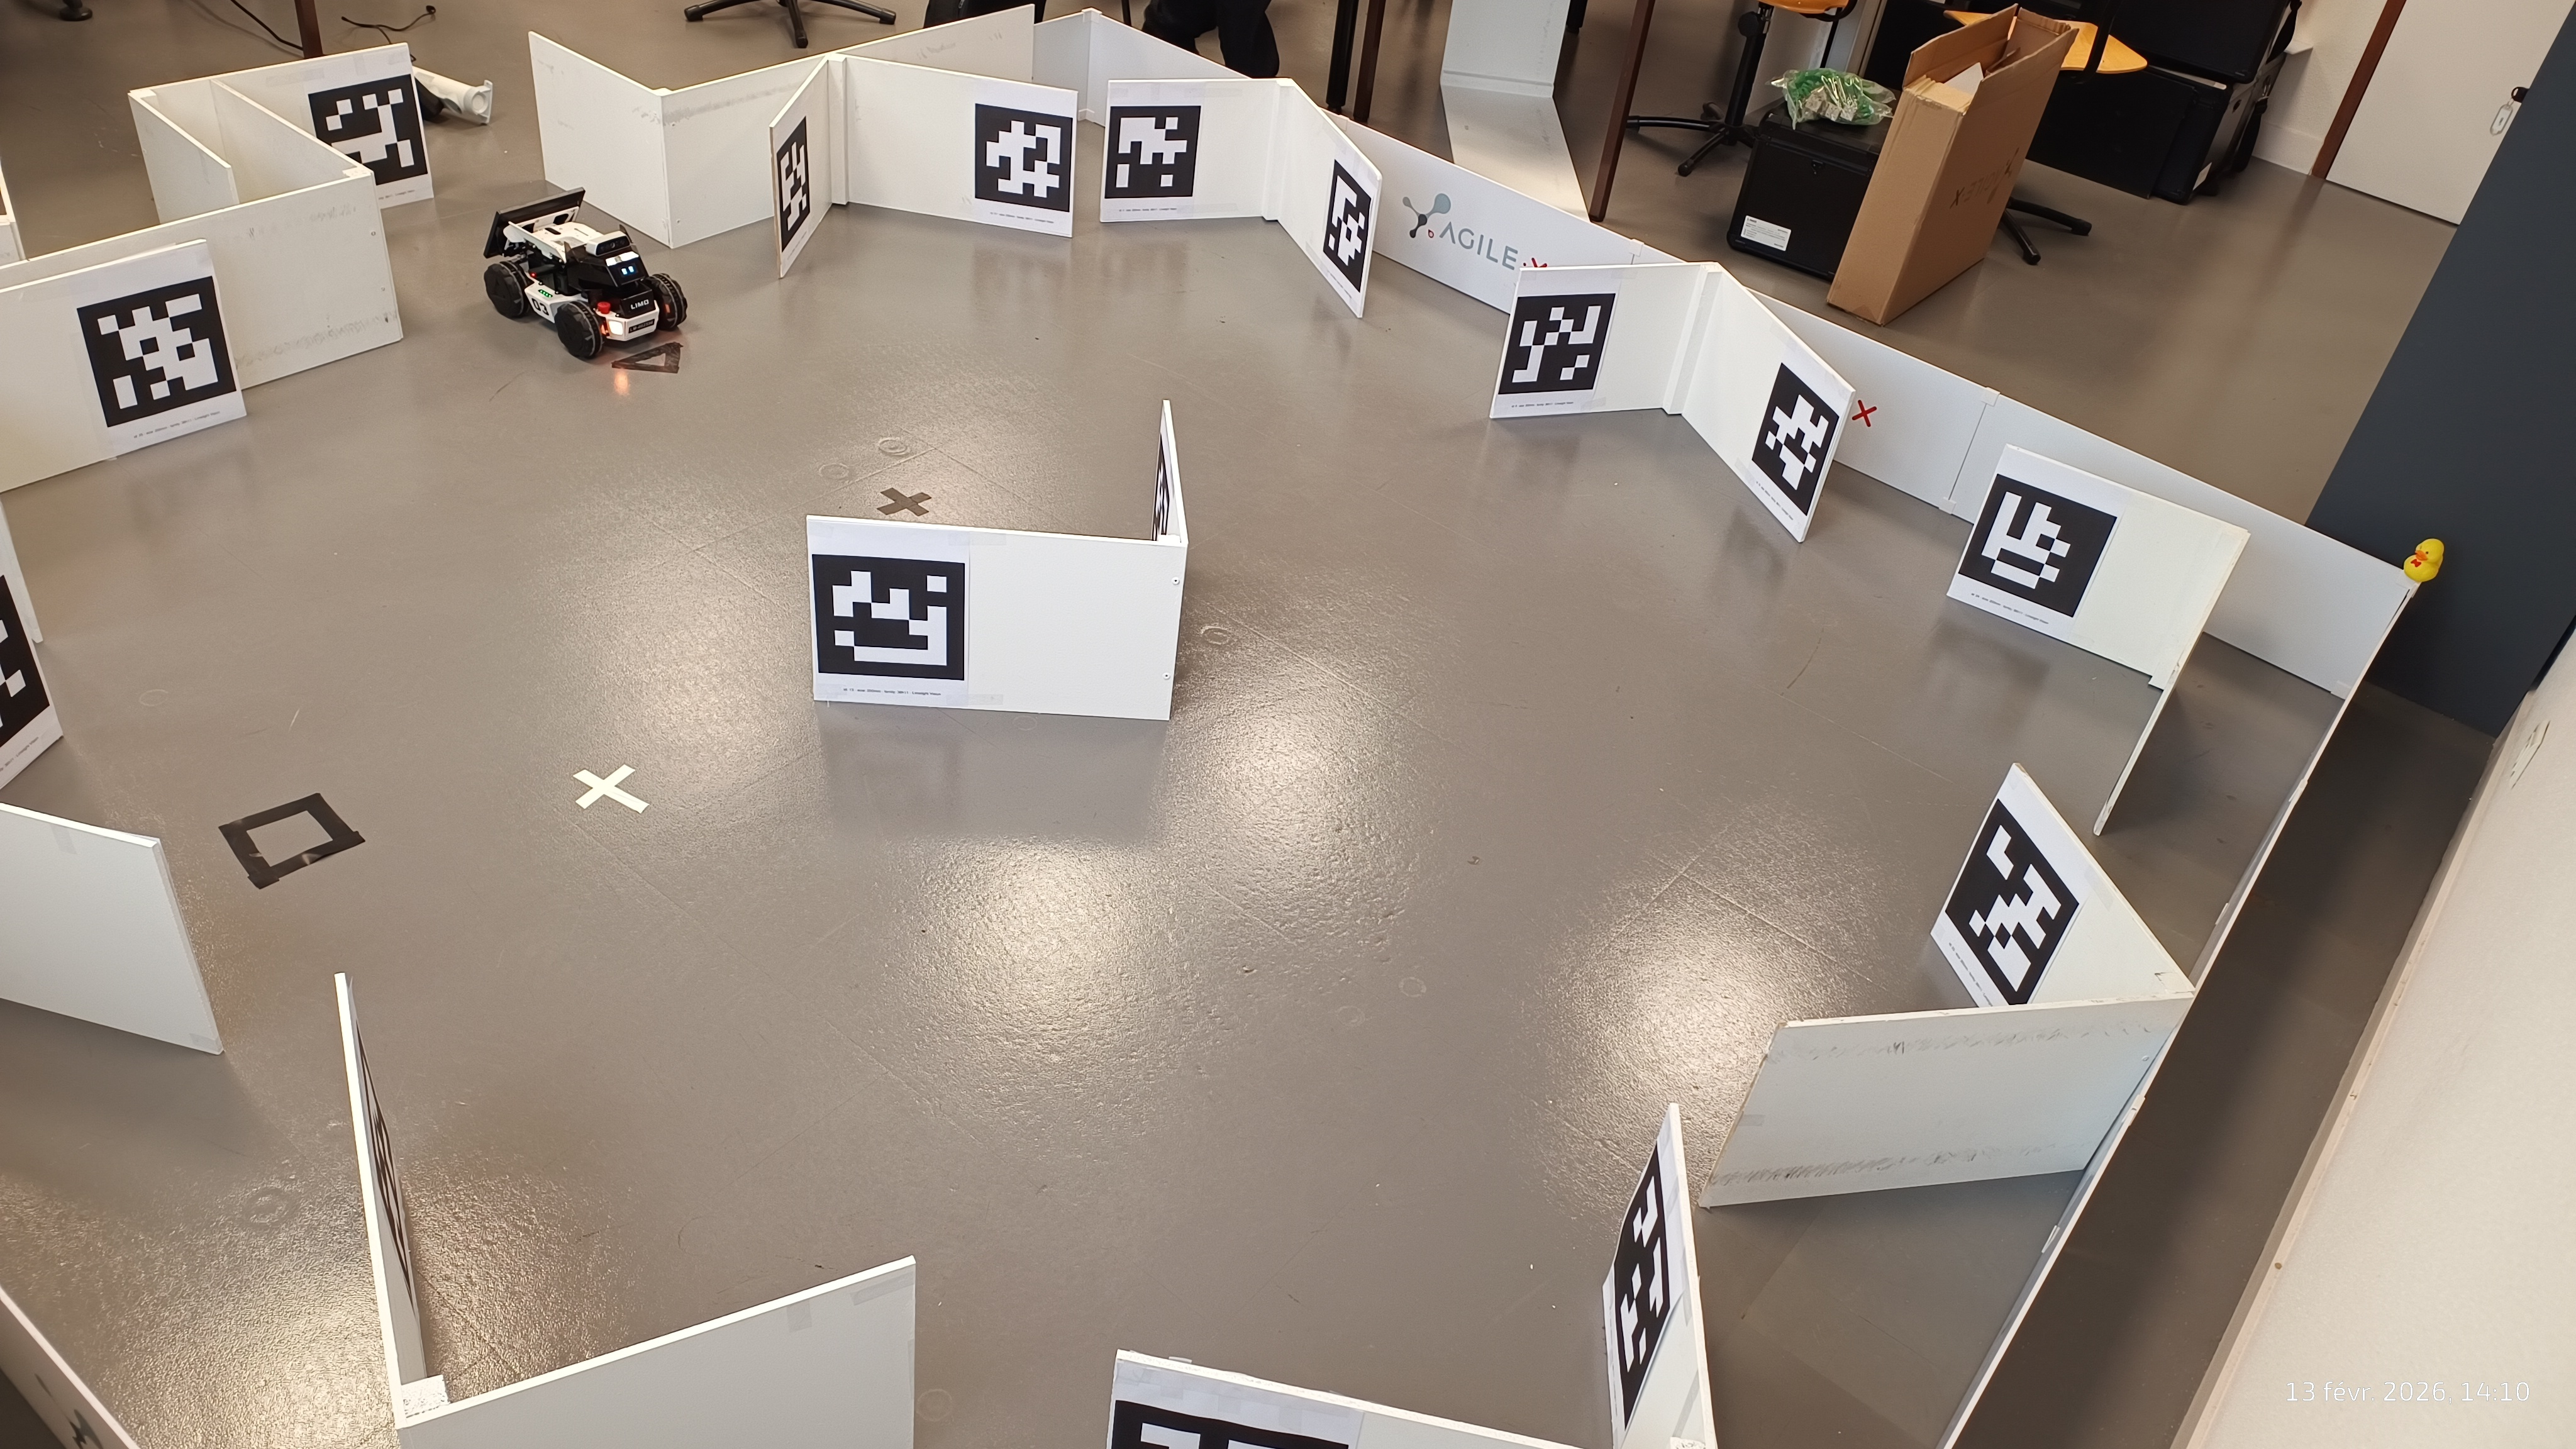
\includegraphics[width=\linewidth,height=0.65\textheight,keepaspectratio]{../Report/Images/recording_fase.jpg}
    \end{column}
    \begin{column}{0.49\textwidth}
      \centering
      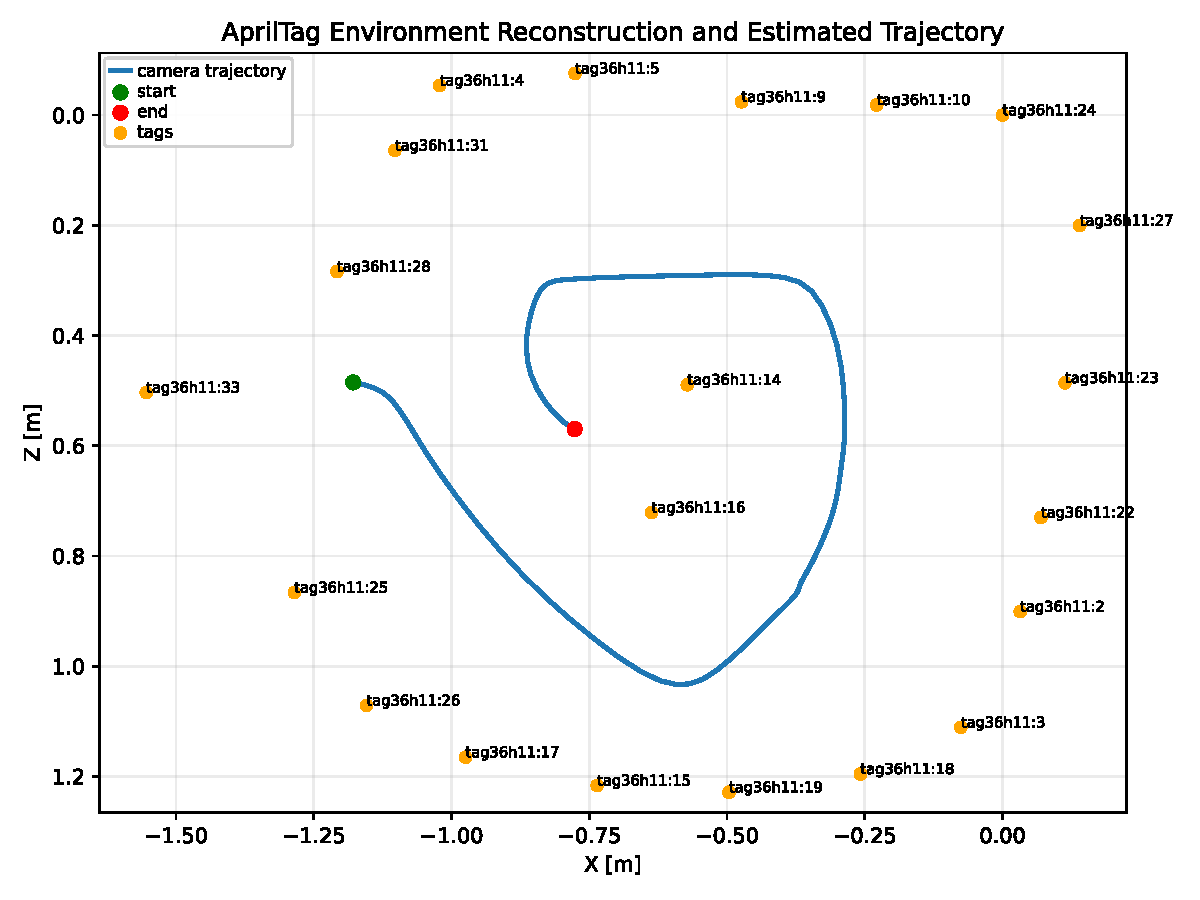
\includegraphics[width=\linewidth,height=0.65\textheight,keepaspectratio]{../Report/svg-inkscape/mapa_trajetoria_xz_svg-raw.pdf}
    \end{column}
  \end{columns}
\end{frame}

\begin{frame}[label=appendix-mosaic-real-relocal]{Real relocalization validation setup and corresponding distance comparison.}
  \begin{columns}[c,onlytextwidth]
    \begin{column}{0.49\textwidth}
      \centering
      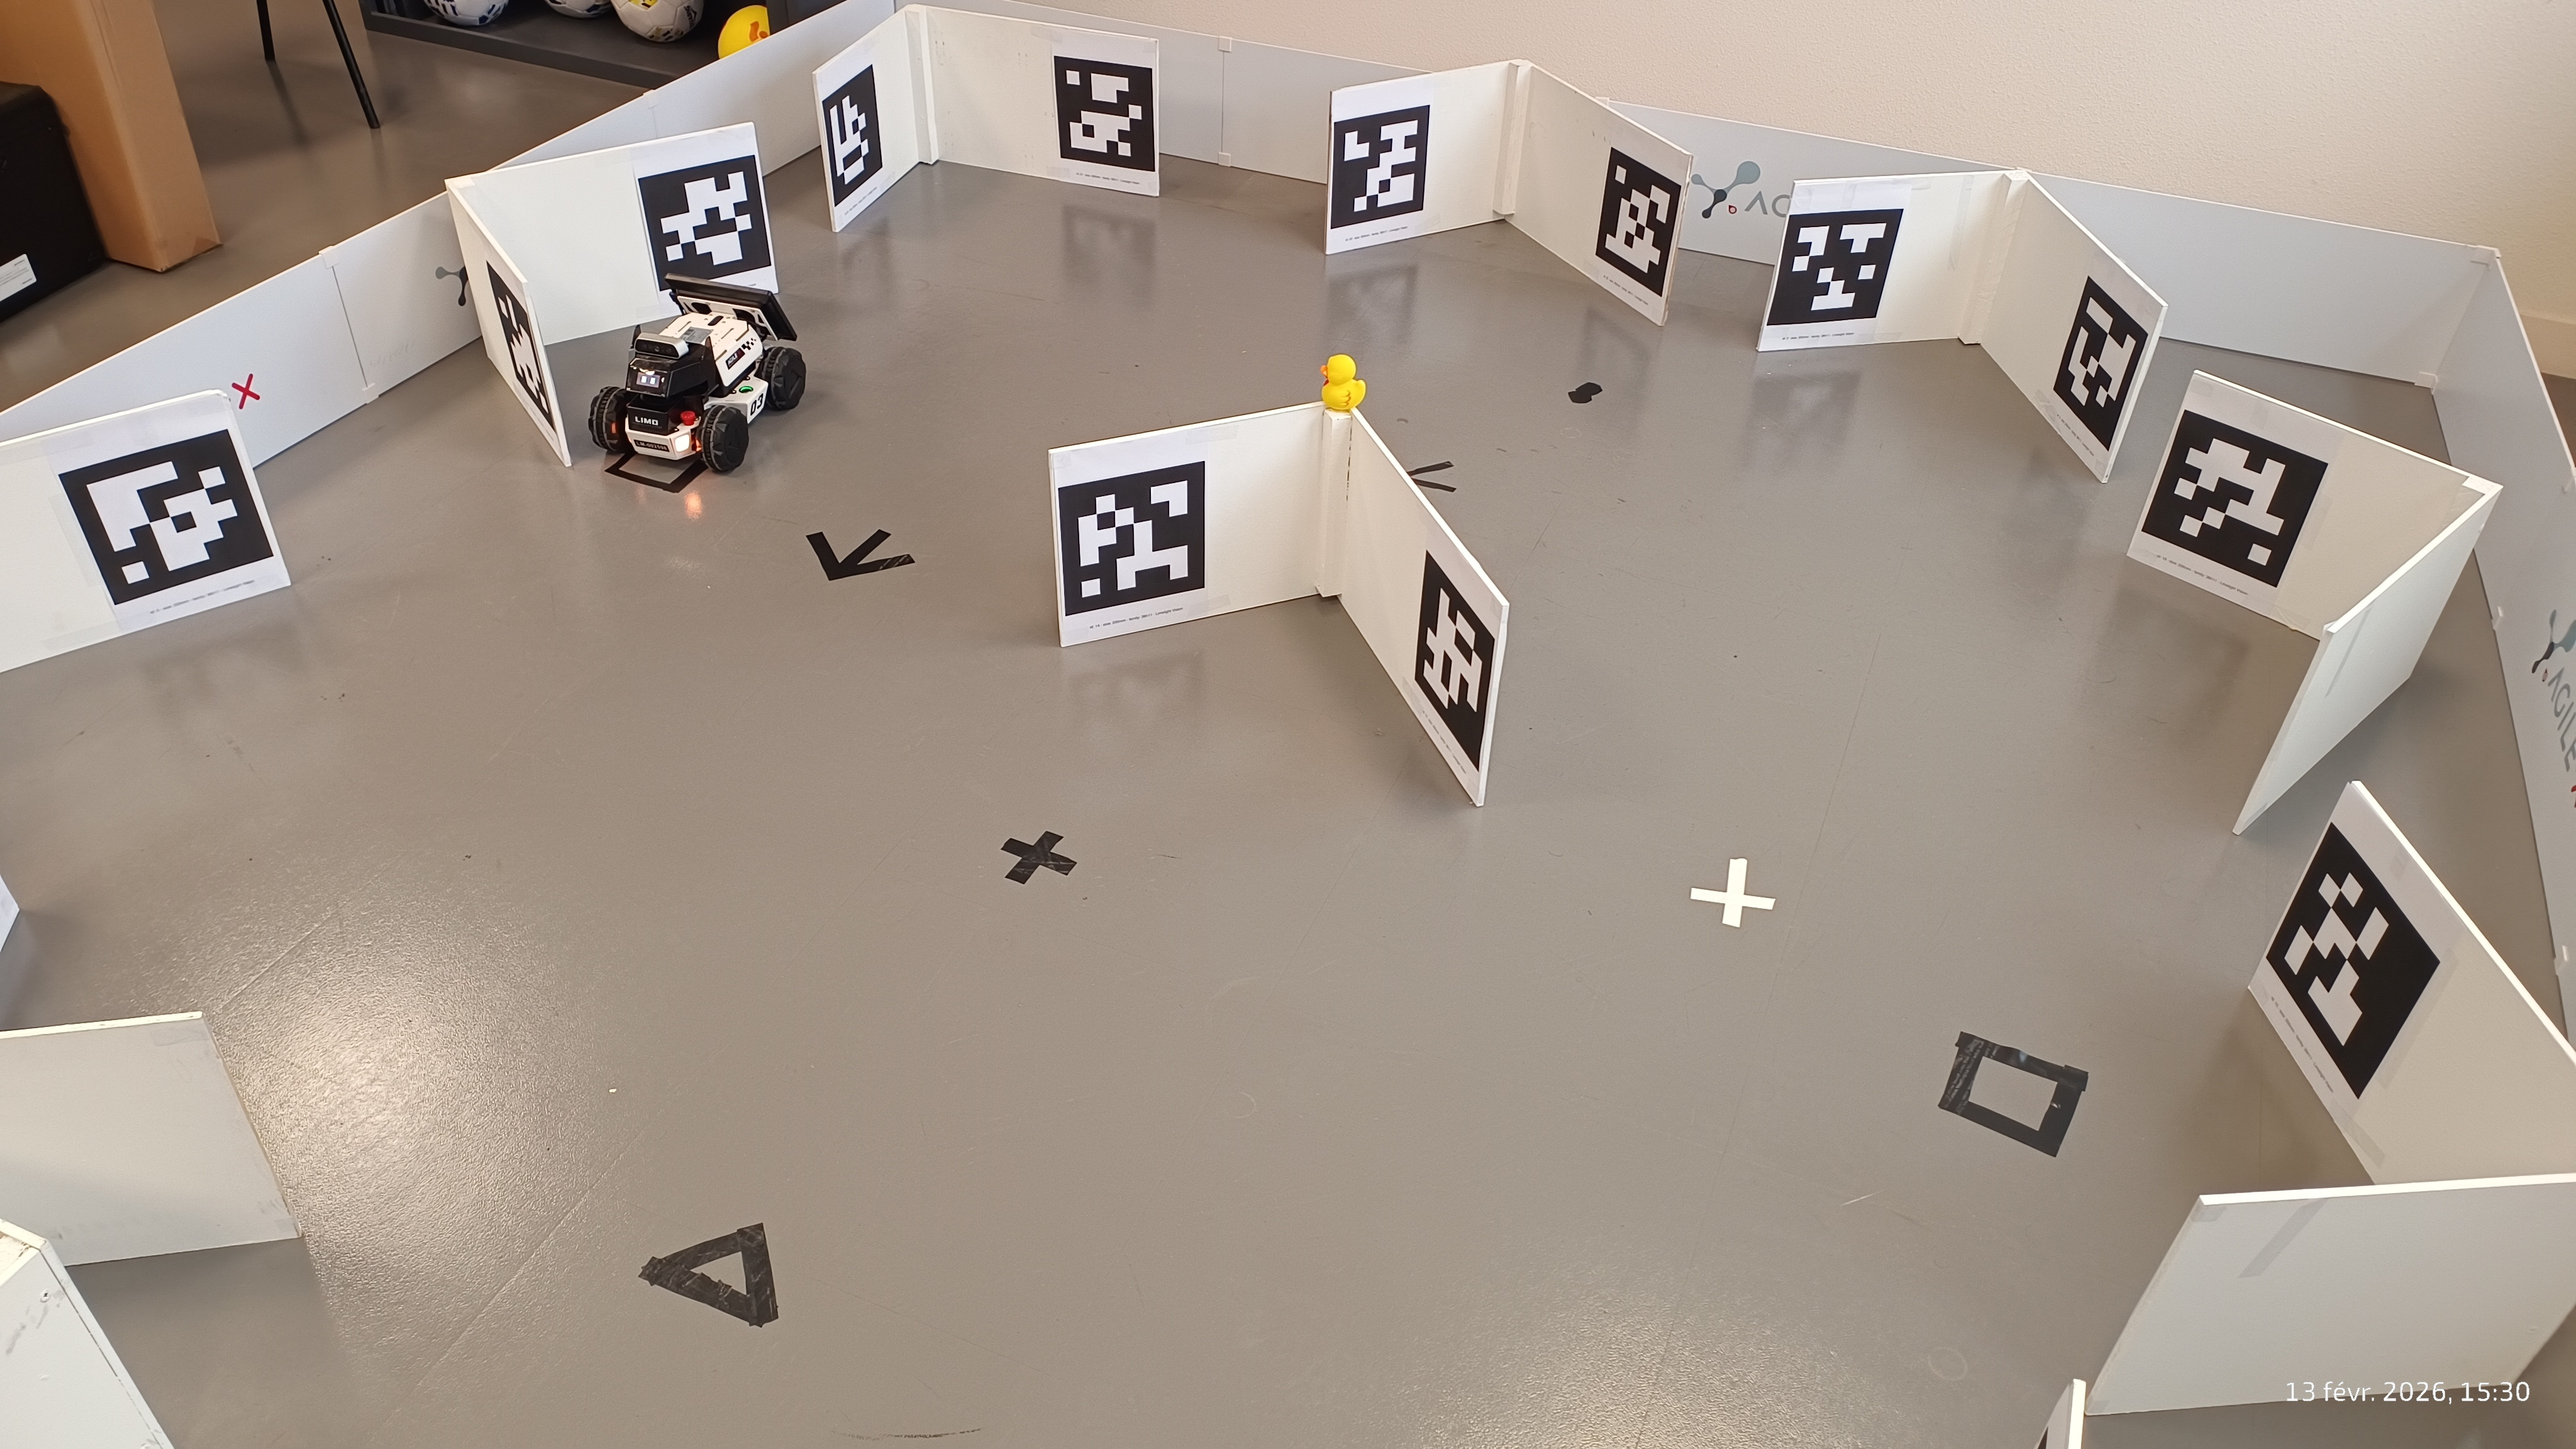
\includegraphics[width=\linewidth,height=0.65\textheight,keepaspectratio]{../Report/Images/relocalization_experiment.jpg}
    \end{column}
    \begin{column}{0.49\textwidth}
      \centering
      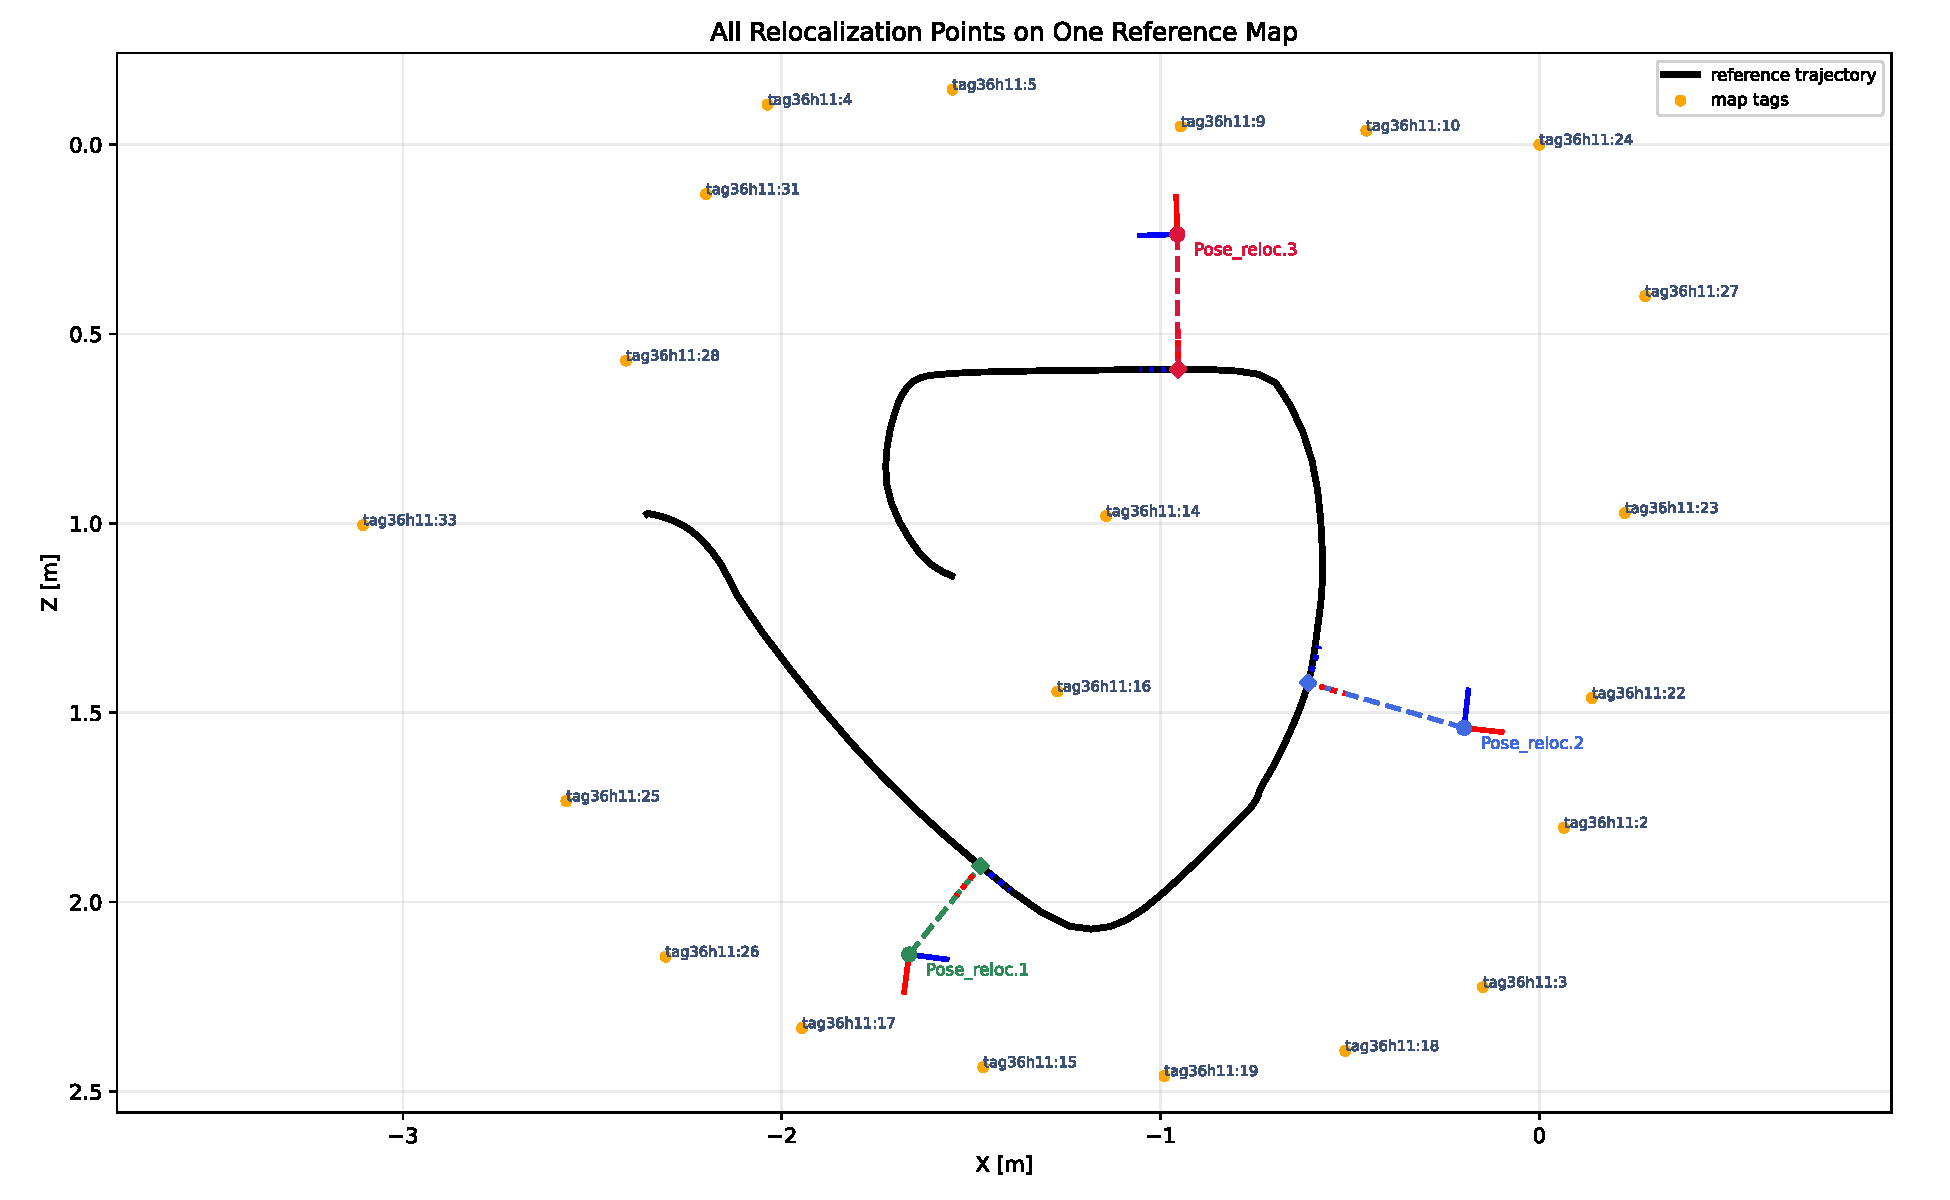
\includegraphics[width=\linewidth,height=0.65\textheight,keepaspectratio]{../Report/svg-inkscape/compare_three_letric_three_cases_points_svg-raw.pdf}
    \end{column}
  \end{columns}
\end{frame}

\begin{frame}[label=appendix-mosaic-second-recording]{Additional real recording result processed with the same offline pipeline.}
  \begin{columns}[c,onlytextwidth]
    \begin{column}{0.49\textwidth}
      \centering
      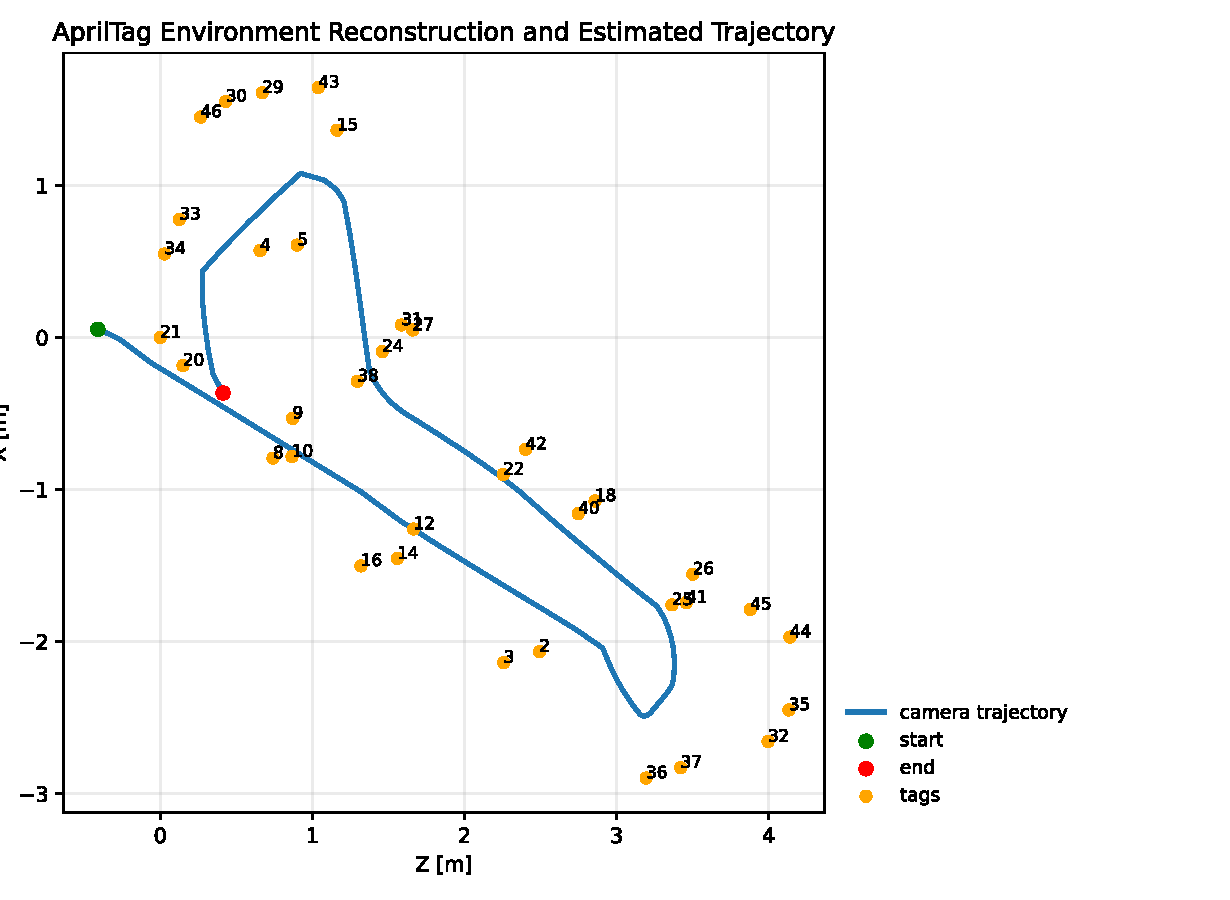
\includegraphics[width=\linewidth,height=0.65\textheight,keepaspectratio]{../Report/Images/output_020_recording_trajectory_basic.pdf}
    \end{column}
    \begin{column}{0.49\textwidth}
      \centering
      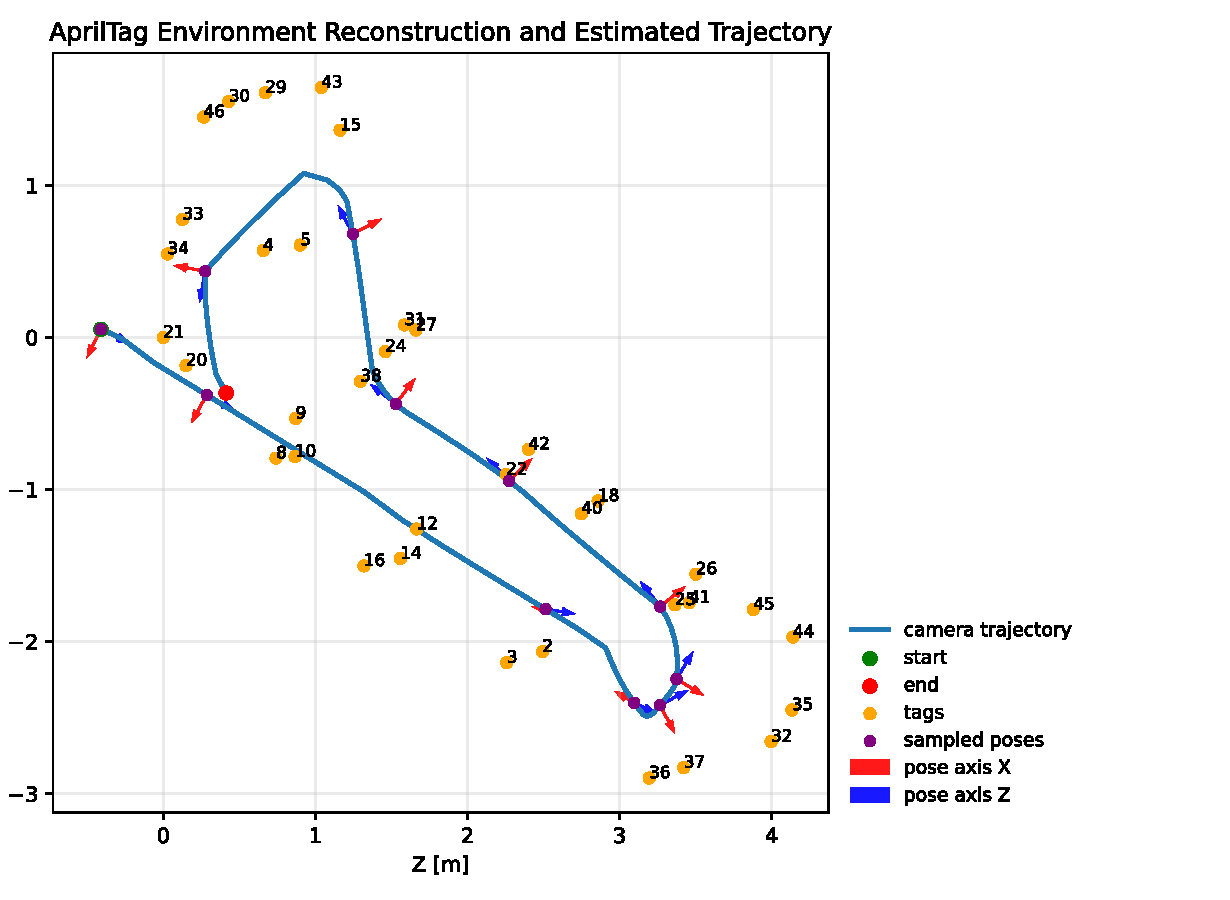
\includegraphics[width=\linewidth,height=0.65\textheight,keepaspectratio]{../Report/Images/output_020_recording_trajectory_with_axes.pdf}
    \end{column}
  \end{columns}
\end{frame}

\begin{frame}[label=appendix-discussion-recording-limitations]{Discussion - Recording Limitations}
\transfade[duration=0.25]
\vspace{-0.08cm}
\begin{outlinecard}[Error Summary Across Validations]
  \scriptsize
  \centering
  \begin{tabular}{lcc}
    \toprule
    \textbf{Validation Case} & \textbf{Traj. Mean Error [m]} & \textbf{Tag/Map Mean Error [m]} \\
    \midrule
    Synthetic (noise-free) & 0.0000 & 0.0000 \\
    Synthetic (+10 cm noise) & 0.0584 & 0.0364 \\
    Simulation & 0.0510 & 0.0873 \\
    Real recording & -- & 0.0390 \\
    \bottomrule
  \end{tabular}
\end{outlinecard}

\vspace{-0.05cm}
\begin{outlinecard}[Reading Notes]
  \small
  \begin{itemize}
    \item Real: map consistency (no full GT).
    \item Sensitive to visibility and calibration.
  \end{itemize}
\end{outlinecard}
\end{frame}

\tikzset{
  appbase/.style={draw=NavyBlue!80, thick, align=center, inner sep=4pt, font=\scriptsize},
  appio/.style={appbase, trapezium, trapezium left angle=70, trapezium right angle=110, fill=AccentBlue!12},
  appproc/.style={appbase, rectangle, rounded corners=1mm, fill=gray!8},
  apppose/.style={appbase, rectangle, rounded corners=1mm, fill=NavyBlue!10},
  appstore/.style={appbase, trapezium, trapezium left angle=70, trapezium right angle=110, fill=gray!8},
  apparrow/.style={-Stealth, thick, draw=NavyBlue!80},
}

\begin{frame}[label=appendix-flowchart-recording]{Architecture of the offline recording pipeline.}
\centering
\resizebox{0.95\linewidth}{!}{
\begin{tikzpicture}[node distance=10mm and 14mm]
  \node[appio] (bag) {Logging dataset\\\textit{rosbag2}};
  \node[appproc, below left=12mm and 6mm of bag] (det) {Detections\\AprilTag};
  \node[appproc, below right=12mm and 6mm of bag] (cam) {Camera intrinsics\\Camera\_Info};
  \node[apppose, right=18mm of bag] (pnp) {\textbf{(1)} Pose estimation (PnP)};
  \node[appproc, right=12mm of pnp] (pair) {\textbf{(2)} Pairwise constraints};
  \node[apppose, right=12mm of pair] (map) {\textbf{(3)} Tag map optimization};
  \node[apppose, below=10mm of map] (traj) {\textbf{(4)} Reference trajectory\\(+ smoothing)};
  \node[appstore, right=12mm of map] (out) {Exports\\tag\_map.yaml/csv\\trajetoria\_camera.csv};
  \draw[apparrow] (det) -- (bag);
  \draw[apparrow] (cam) -- (bag);
  \draw[apparrow] (bag) -- (pnp);
  \draw[apparrow] (pnp) -- (pair);
  \draw[apparrow] (pair) -- (map);
  \draw[apparrow] (map) -- (out);
  \draw[apparrow] (map) -- (traj);
  \draw[apparrow] (traj.east) -| (out.south);
\end{tikzpicture}
}
\end{frame}

\begin{frame}[label=appendix-flowchart-relocal]{Architecture of the relocalization pipeline with separated offline analysis and online execution.}
\centering
\resizebox{0.95\linewidth}{!}{
\begin{tikzpicture}[node distance=10mm and 12mm]
  \node[appstore] (reftraj) {Reference trajectory\\trajetoria\_camera.csv};
  \node[appstore, right=12mm of reftraj] (refmap) {Tag map\\tag\_map.yaml/csv};
  \node[appio, below=14mm of reftraj] (qoff) {Query poses\\(offline dataset)};
  \node[appproc, right=10mm of qoff] (align) {\textbf{(1)} Optional planar\\alignment};
  \node[apppose, right=10mm of align] (nearoff) {\textbf{(2)} Nearest point\\search};
  \node[apppose, right=10mm of nearoff] (erroff) {\textbf{(3)} Compute\\$D$ and $\phi$};
  \node[appstore, right=10mm of erroff] (report) {Exports\\metrics/plots};
  \node[appio, below=12mm of qoff] (live) {Estimated robot pose\\(online)};
  \node[appproc, right=10mm of live] (load) {\textbf{(4*)} Load\\reference};
  \node[apppose, right=10mm of load] (nearon) {\textbf{(5)} Nearest\\point+tangent};
  \node[apppose, right=10mm of nearon] (erron) {\textbf{(6)} Output\\$D$ and $\phi$};
  \node[appstore, right=10mm of erron] (topics) {ROS topics\\distance, heading};
  \draw[apparrow] (reftraj.south) -- (qoff.north);
  \draw[apparrow] (refmap.south) -- (align.north);
  \draw[apparrow] (qoff) -- (align) -- (nearoff) -- (erroff) -- (report);
  \draw[apparrow] (live) -- (load) -- (nearon) -- (erron) -- (topics);
\end{tikzpicture}
}
\end{frame}

\begin{frame}[label=appendix-table-20]{Table 2.0: Functional Requirements}
\scriptsize
\centering
\begin{tabular}{|c|p{0.79\linewidth}|}
\hline
\textbf{ID} & \textbf{Requirement} \\ \hline
FR1 & The system shall provide workflows for recording robot motion and perception data into rosbag2 datasets for offline processing. \\ \hline
FR2 & The system shall process recorded rosbag2 datasets offline to generate a reference trajectory and a spatial map of detected AprilTags. \\ \hline
FR3 & The offline processing stage shall export structured output files, including trajectory CSV and tag map YAML/CSV formats. \\ \hline
FR4 & The system shall provide an online relocalization node capable of loading a reference trajectory, subscribing to a live pose topic, computing nearest-point distance and heading deviation, and publishing these quantities for controller integration. \\ \hline
FR5 & The system shall publish visualization-compatible ROS topics enabling RViz display of reference trajectory, current pose, nearest reference pose, and relocalization error indicators. \\ \hline
FR6 & The system shall provide launch files and profile scripts supporting both real and simulation workflows. \\ \hline
FR7 & The system shall include documented execution procedures ensuring reproducibility from recorded datasets. \\ \hline
\end{tabular}
\end{frame}

\begin{frame}[label=appendix-table-21]{Table 2.1: Non-Functional Requirements}
\scriptsize
\centering
\begin{tabular}{|c|p{0.79\linewidth}|}
\hline
\textbf{ID} & \textbf{Requirement} \\ \hline
NFR1 & Offline reconstruction shall be executable independently of live robot operation. \\ \hline
NFR2 & Online relocalization shall operate within computational limits compatible with real-time ROS~2 execution. \\ \hline
NFR3 & The architecture shall maintain separation between perception, offline reconstruction, and online relocalization components. \\ \hline
NFR4 & The system shall ensure consistency of coordinate frames within the ROS~2 TF structure. \\ \hline
NFR5 & Dataset files shall remain external to version control to maintain repository portability. \\ \hline
\end{tabular}
\end{frame}

\begin{frame}[label=appendix-table-22]{Table 2.2: Project Deliverables and Constraints}
\scriptsize
\centering
\begin{tabular}{|c|p{0.79\linewidth}|}
\hline
\textbf{ID} & \textbf{Requirement} \\ \hline
PR1 & The project shall be delivered as a version-controlled ROS~2 workspace repository containing source code, launch files, scripts, and documentation. \\ \hline
PR2 & The repository shall include structured workflows for both real and simulation execution. \\ \hline
C1 & The system shall be implemented in ROS~2 Humble. \\ \hline
C2 & The perception pipeline shall use AprilTag v3 with the tag36h11 family. \\ \hline
C3 & Experimental validation shall be conducted on the AgileX LIMO platform. \\ \hline
C4 & The system shall not include full autonomous navigation, SLAM of unknown environments, obstacle avoidance, or mission-level planning. \\ \hline
\end{tabular}
\end{frame}

\begin{frame}[label=appendix-table-23]{Table 2.3: Technical Limitations}
\scriptsize
\centering
\begin{tabular}{|c|p{0.79\linewidth}|}
\hline
\textbf{ID} & \textbf{Limitation} \\ \hline
TL1 & Accurate and stable pose estimation assumes that at least two AprilTags are simultaneously visible in the camera field of view. While pose can be computed from a single detection, multi-tag observations improve numerical stability and reduce sensitivity to noise and calibration errors. \\ \hline
TL2 & Localization precision depends on camera calibration quality, tag size, distance to the tags, and image resolution. The system does not guarantee fixed absolute accuracy under arbitrary environmental conditions. \\ \hline
\end{tabular}
\end{frame}

\begin{frame}[label=appendix-table-41]{Table 4.1: Residual errors in the ideal scenario (no noise).}
\small
\centering
\begin{tabular}{|l|c|c|c|}
\hline
\textbf{Metric} & \textbf{Mean Error} & \textbf{Minimum} & \textbf{Maximum} \\ \hline
Camera Trajectory & $0.0000\text{ m} / 0.00^\circ$ & $0.0000\text{ m} / 0.00^\circ$ & $0.0000\text{ m} / 0.00^\circ$ \\ \hline
Tag Poses & $0.0000\text{ m} / 0.00^\circ$ & $0.0000\text{ m} / 0.00^\circ$ & $0.0000\text{ m} / 0.00^\circ$ \\ \hline
\end{tabular}
\end{frame}

\begin{frame}[label=appendix-table-42]{Table 4.2: Error statistics under 10 cm Gaussian noise.}
\small
\centering
\begin{tabular}{|l|c|c|c|}
\hline
\textbf{Metric} & \textbf{Mean Error} & \textbf{Minimum} & \textbf{Maximum} \\ \hline
Camera Trajectory & $0.0584\text{ m} / 0.97^\circ$ & $0.0126\text{ m} / 0.11^\circ$ & $0.1485\text{ m} / 2.67^\circ$ \\ \hline
Tag Poses & $0.0364\text{ m} / 0.73^\circ$ & $0.0156\text{ m} / 0.73^\circ$ & $0.0583\text{ m} / 0.73^\circ$ \\ \hline
\end{tabular}
\end{frame}

\begin{frame}[label=appendix-table-43]{Table 4.3: Summary table with estimated versus measured distance to the recorded trajectory and the estimated heading offset $\phi$.}
\small
\centering
\begin{tabular}{|c|c|c|c|c|}
\hline
\textbf{Relocalization Case} & \textbf{Estimated D [m]} & \textbf{Measured D [m]} & \textbf{Error [m]} & \textbf{$\phi$ [deg]} \\ \hline
1 & 0.2998 & 0.3100 & 0.0102 & -31.38 \\ \hline
2 & 0.4284 & 0.4200 & 0.0084 & -10.34 \\ \hline
3 & 0.3567 & 0.3600 & 0.0033 & -1.63 \\ \hline
\end{tabular}
\end{frame}

\begin{frame}[label=appendix-table-a1]{Table A.1: Comparison between estimated and measured distances from tag 16.}
\tiny
\centering
\scalebox{0.68}{%
\begin{tabular}{|c|c|c|c|c|}
\hline
\textbf{Source tag} & \textbf{Target tag} & \textbf{Estimated [m]} & \textbf{Measured [m]} & \textbf{Absolute error [m]} \\ \hline
16 & 2 & 1.385 & 1.380 & 0.005 \\ \hline
16 & 3 & 1.368 & 1.360 & 0.008 \\ \hline
16 & 4 & 1.728 & 1.820 & 0.092 \\ \hline
16 & 5 & 1.613 & 1.690 & 0.077 \\ \hline
16 & 9 & 1.527 & 1.450 & 0.077 \\ \hline
16 & 10 & 1.691 & 1.680 & 0.011 \\ \hline
16 & 14 & 0.481 & 0.480 & 0.001 \\ \hline
16 & 15 & 1.011 & 1.110 & 0.099 \\ \hline
16 & 17 & 1.115 & 1.090 & 0.025 \\ \hline
16 & 18 & 1.216 & 1.220 & 0.004 \\ \hline
16 & 19 & 1.054 & 1.040 & 0.014 \\ \hline
16 & 22 & 1.412 & 1.410 & 0.002 \\ \hline
16 & 23 & 1.571 & 1.560 & 0.011 \\ \hline
16 & 24 & 1.925 & 1.900 & 0.025 \\ \hline
16 & 25 & 1.328 & 1.300 & 0.028 \\ \hline
16 & 26 & 1.249 & 1.220 & 0.029 \\ \hline
16 & 27 & 1.871 & 1.800 & 0.071 \\ \hline
16 & 28 & 1.436 & 1.470 & 0.034 \\ \hline
16 & 31 & 1.608 & 1.660 & 0.052 \\ \hline
16 & 33 & 1.886 & 1.870 & 0.016 \\ \hline
\textbf{Mean} & - & - & - & \textbf{0.039} \\ \hline
\textbf{Max} & - & - & - & \textbf{0.099} \\ \hline
\textbf{Min} & - & - & - & \textbf{0.001} \\ \hline
\end{tabular}
}
\end{frame}

\edef\MediaRelocDemoOneFile{\detokenize{assets/reloc_demo1.webm}}
\edef\MediaRelocDemoTwoFile{\detokenize{assets/reloc_demo2.webm}}
\edef\MediaRelocRealScenarioOneFile{\detokenize{assets/reloc_real_scneario_1.webm}}
\edef\MediaRelocScenarioTwoFile{\detokenize{assets/Reloc_scnerio2.webm}}
\edef\MediaTrajectoryOneFile{\detokenize{assets/trajetory_1_4x_cropped.mp4}}
\edef\MediaRelocDemoOneThumb{\detokenize{assets/media_reloc_demo1_thumb.jpg}}
\edef\MediaRelocDemoTwoThumb{\detokenize{assets/media_reloc_demo2_thumb.jpg}}
\edef\MediaRelocRealScenarioOneThumb{\detokenize{assets/media_reloc_real1_thumb.jpg}}
\edef\MediaRelocScenarioTwoThumb{\detokenize{assets/media_reloc_scn2_thumb.jpg}}
\edef\MediaTrajectoryOneThumb{\detokenize{assets/media_traj1_thumb.jpg}}
\edef\MediaValidationExpTwoFile{\detokenize{assets/trajetory_2_5x_cropped.mp4}}
\edef\MediaValidationExpTwoThumb{\detokenize{assets/trajetory_2_thumb.jpg}}

\begin{frame}[label=appendix-media-validation-exp2]{Appendix Media - Validation Experiment 2 (Large)}
\centering
\vspace{0.05cm}
\IfFileExists{\MediaValidationExpTwoFile}{
  \movie[
    width=0.60\linewidth,
    height=0.45\linewidth,
    poster
  ]{%
    \fcolorbox{NavyBlue}{white}{%
      \includegraphics[
        width=\dimexpr0.60\linewidth-2\fboxrule\relax,
        height=\dimexpr0.45\linewidth-2\fboxrule\relax,
        keepaspectratio
      ]{\MediaValidationExpTwoThumb}%
    }%
  }{\MediaValidationExpTwoFile}
}{
  \begin{alertbox}[Video Missing]
    Add the file \texttt{\MediaValidationExpTwoFile}.
  \end{alertbox}
}
\end{frame}

\begin{frame}[label=appendix-media-reloc-demo1]{Appendix Media - reloc\_demo1.webm}
\centering
\IfFileExists{\MediaRelocDemoOneFile}{
  \movie[
    width=0.92\linewidth,
    height=0.24\linewidth,
    poster
  ]{%
    \fcolorbox{NavyBlue}{white}{\includegraphics[width=\linewidth,height=0.24\linewidth,keepaspectratio]{\MediaRelocDemoOneThumb}}%
  }{\MediaRelocDemoOneFile}
}{
  \begin{alertbox}[Video Missing]
    Add the file \texttt{\MediaRelocDemoOneFile}.
  \end{alertbox}
}
\end{frame}

\begin{frame}[label=appendix-media-reloc-demo2]{Appendix Media - reloc\_demo2.webm}
\centering
\IfFileExists{\MediaRelocDemoTwoFile}{
  \movie[
    width=0.92\linewidth,
    height=0.24\linewidth,
    poster
  ]{%
    \fcolorbox{NavyBlue}{white}{\includegraphics[width=\linewidth,height=0.24\linewidth,keepaspectratio]{\MediaRelocDemoTwoThumb}}%
  }{\MediaRelocDemoTwoFile}
}{
  \begin{alertbox}[Video Missing]
    Add the file \texttt{\MediaRelocDemoTwoFile}.
  \end{alertbox}
}
\end{frame}

\begin{frame}[label=appendix-media-reloc-real1]{Appendix Media - reloc\_real\_scneario\_1.webm}
\centering
\IfFileExists{\MediaRelocRealScenarioOneFile}{
  \movie[
    width=0.92\linewidth,
    height=0.43\linewidth,
    poster
  ]{%
    \fcolorbox{NavyBlue}{white}{\includegraphics[width=\linewidth,height=0.43\linewidth,keepaspectratio]{\MediaRelocRealScenarioOneThumb}}%
  }{\MediaRelocRealScenarioOneFile}
}{
  \begin{alertbox}[Video Missing]
    Add the file \texttt{\MediaRelocRealScenarioOneFile}.
  \end{alertbox}
}
\end{frame}

\begin{frame}[label=appendix-media-reloc-scn2]{Appendix Media - Reloc\_scnerio2.webm}
\centering
\IfFileExists{\MediaRelocScenarioTwoFile}{
  \movie[
    width=0.92\linewidth,
    height=0.43\linewidth,
    poster
  ]{%
    \fcolorbox{NavyBlue}{white}{\includegraphics[width=\linewidth,height=0.43\linewidth,keepaspectratio]{\MediaRelocScenarioTwoThumb}}%
  }{\MediaRelocScenarioTwoFile}
}{
  \begin{alertbox}[Video Missing]
    Add the file \texttt{\MediaRelocScenarioTwoFile}.
  \end{alertbox}
}
\end{frame}

\begin{frame}[label=appendix-media-traj1]{Appendix Media - trajetory\_1\_4x\_cropped.mp4}
\centering
\IfFileExists{\MediaTrajectoryOneFile}{
  \movie[
    width=0.92\linewidth,
    height=0.44\linewidth,
    poster
  ]{%
    \fcolorbox{NavyBlue}{white}{\includegraphics[width=\linewidth,height=0.44\linewidth,keepaspectratio]{\MediaTrajectoryOneThumb}}%
  }{\MediaTrajectoryOneFile}
}{
  \begin{alertbox}[Video Missing]
    Add the file \texttt{\MediaTrajectoryOneFile}.
  \end{alertbox}
}
\end{frame}
